% Quelle der Übersetzung: Schneefl0cke https://www.fanfiktion.de/s/60044849000ccc541aef297e/121/
% \chapter{Something to Protect: Hermione Granger}
\chapter{Was sich zu beschützen lohnt: Hermine Granger}

% \lettrinepara{A}{nd} it was evening and it was morning, the last day. June 15th, 1992.
\lettrinepara{U}{nd} es war Abend und es war Morgen, der letzte Tag. 15. Juni 1992.

\hplettrineextrapara
% The beginning light of morning, the pre-dawn before sunrise, was barely brightening the sky. To the east of Hogwarts, where the Sun would rise, that faintest tinge of grey made barely visible the hilly horizon beyond the Quidditch stands.
Das beginnende Licht des Morgens, die Vor-Dämmerung vor dem Sonnenaufgang, erhellte den Himmel kaum. Östlich von Hogwarts, wo die Sonne aufgehen würde, machte dieser schwache Grauton den hügeligen Horizont jenseits der Quidditch-Tribüne kaum sichtbar.
% The stone terrace-platform where Harry now sat would be high enough to see the dawn beyond the hills below; he’d asked for that, when he was describing his new office.
Die steinerne Terrassenplattform, auf der Harry jetzt saß, würde hoch genug sein, um die Morgendämmerung jenseits der Hügel zu sehen; das hatte er sich gewünscht, als er sein neues Büro beschrieben hatte.
% Harry was currently sitting cross-legged on a cushion, chilly pre-morning breezes stirring over his exposed hands and face. He’d ordered the house elves to bring up the hand-glittered throne from his previous office as General Chaos…and then he’d told the elves to put it back, once it had occurred to Harry to start worrying about where his taste in decorations had come from and whether Voldemort had once possessed a similar throne. Which, itself, wasn’t a knockdown argument—it wasn’t like sitting on a glittery throne to survey the lands below Hogwarts was \emph{unethical} in any way Harry’s moral philosophy could make out—but Harry had decided that he needed to take time and think it through. Meanwhile, simple cushions would do well enough.
Harry saß gerade im Schneidersitz auf einem Kissen, eine kühle Morgenbrise strich über seine ungeschützten Hände und sein Gesicht. Er hatte den Hauselfen befohlen, den handgeschmückten Thron aus seinem früheren Büro als General Chaos heraufzuholen…und dann hatte er den Elfen gesagt, sie sollten ihn wieder zurückbringen, nachdem es Harry in den Sinn gekommen war, sich Gedanken darüber zu machen, woher sein Geschmack für Innendekorationen stammte und ob Voldemort einst einen ähnlichen Thron besessen hatte. Was an sich kein schlagendes Argument war—es war ja nicht so, dass das Sitzen auf einem glitzernden Thron, um die Ländereien unterhalb von Hogwarts zu überblicken, in irgendeiner Weise unethisch war, wie Harrys Moralphilosophie es erkennen konnte—, aber Harry hatte beschlossen, dass er sich Zeit nehmen und es durchdenken musste. In der Zwischenzeit würden einfache Kissen genügen.

% In the room below, connected to the rooftop by a simple wooden ladder, was Harry’s new office inside Hogwarts. A wide room, surrounded by full-wall windows on four sides for sunlight; currently bare of furnishings but for four chairs and a desk. Harry had told Headmistress McGonagall what he was looking for, and Headmistress McGonagall had put on the Sorting Hat and then told Harry the series of twists and turns that would take him where he wanted to be. High enough in Hogwarts that the castle shouldn’t have been that tall, high enough in Hogwarts that nobody looking from the outside would see a piece of castle corresponding to where Harry now sat. It seemed like an elementary precaution against snipers that there was no reason \emph{not} to take.
Im Raum darunter, der durch eine einfache Holzleiter mit dem Dach verbunden war, befand sich Harrys neues Büro in Hogwarts. Ein großer Raum, der auf vier Seiten von Fenstern umgeben war, die das Sonnenlicht hereinließen, und der bis auf vier Stühle und einen Schreibtisch noch nicht eingerichtet war. Harry hatte Schulleiterin McGonagall gesagt, was er suchte, und Schulleiterin McGonagall hatte den Sprechenden Hut aufgesetzt und Harry dann die Reihe von Drehungen und Wendungen erklärt, die ihn dorthin bringen würden, wo er sein wollte. Hoch genug in Hogwarts, dass das Schloss nicht so hoch sein sollte, hoch genug in Hogwarts, dass niemand, der von außen hinsah, ein Stück des Schlosses sehen würde, das dem entsprach, wo Harry jetzt saß. Es schien eine elementare Vorsichtsmaßnahme gegen Scharfschützen zu sein, gegen die es keinen Grund gab, sie \emph{nicht} zu treffen.

% Though, on the flip side, Harry had no idea where he currently \emph{was} in any real sense. If his office couldn’t be seen from the lands below, then how was Harry seeing the lands, how were photons making it from the landscape to him? On the western side of the horizon, stars still glittered, clear in the pre-dawn air. Were those photons the actual photons that had been emitted by huge plasma furnaces in the unimaginable distance? Or did Harry now sit within some dreaming vision of the Hogwarts castle? Or was it all, without any further explanation, ‘just magic’? He needed to get electricity to work better around magic so he could experiment with shining lasers downward and upward.
Andererseits hatte Harry aber auch keine Ahnung, wo er sich im Moment wirklich befand. Wenn sein Büro vom Boden aus nicht zu sehen war, wie konnte Harry dann den Boden sehen, wie schafften es Photonen von der Landschaft zu ihm?
Auf der westlichen Seite des Horizonts glitzerten immer noch Sterne, klar in der Luft vor der Morgendämmerung. Waren diese Photonen die tatsächlichen Photonen, die von riesigen Plasmaöfen in der unvorstellbaren Ferne ausgestoßen worden waren? Oder saß Harry jetzt in einer träumerischen Vision des Schlosses Hogwarts? Oder war das alles, ohne weitere Erklärung, „nur Magie“? Er musste die Elektrizität dazu bringen, besser mit der Magie umzugehen, damit er mit dem Abwärts- und Aufwärtsstrahlen von Lasern experimentieren konnte.

% And yes, Harry had his own office on Hogwarts now. He didn’t have any official title yet, but the Boy-Who-Lived was now a true fixture of the Hogwarts School of Witchcraft and Wizardry, the soon-to-be-home of the Philosopher’s Stone and the world’s only wizarding institution of genuinely higher education. It wasn’t fully secured, but Professor Vector had put up some preliminary Charms and Runes to screen the office and its rooftop against eavesdropping.
Und ja, Harry hatte jetzt sein eigenes Büro auf Hogwarts. Er hatte zwar noch keinen offiziellen Titel, aber der Junge-der-überlebte war jetzt ein fester Bestandteil der Hogwarts-Schule für Hexerei und Zauberei, der baldigen Heimat des Steins der Weisen und der einzigen höheren Bildungseinrichtung der Welt für Zauberer. Es war nicht vollständig gesichert, aber Professor Vector hatte einige vorläufige Zaubersprüche und Runen angebracht, um das Büro und sein Dach gegen Lauschangriffe abzuschirmen.

% Harry sat on his cushion, near the edge of his office’s roof, and gazed down upon trees and lakes and flowering grass. Far below, carriages sat motionlessly, not yet harnessed to skeletal horses. Small boats littered the shore, prepared to ferry younger students across the lake when the time came. The Hogwarts Express had arrived overnight, and now the carriages and the huge old-fashioned engine awaited on the other side of the southern lake. All was ready to take the students home after the Leave-Taking Feast in the morning.
Harry saß auf seinem Kissen in der Nähe der Dachkante seines Büros und blickte auf Bäume, Seen und blühendes Gras hinunter. Weit unten saßen bewegungslos Kutschen, die noch nicht an die skelettierten Pferde angeschirrt waren. Kleine Boote lagen am Ufer, bereit, die jüngeren Schüler über den See zu bringen, wenn die Zeit gekommen war. Der Hogwarts-Express war über Nacht angekommen, und nun warteten die Waggons und die riesige altmodische Lokomotive auf der anderen Seite des südlichen Sees. Alles war bereit, um die Schüler nach dem Abschiedsfest am Morgen nach Hause zu bringen.

% Harry stared across the lake, at the great old-fashioned locomotive he wouldn’t be riding home this time. Again. There was a strange sadness and worry to that thought, like Harry was already starting to miss out on the bonding experiences with \emph{the other students his age}—if you could say that at all, when a significant part of Harry had been born in 1926. It had felt to Harry, last night in the Ravenclaw common room, like the gap between him and the other students had, yes, widened even further. Though that might only have been from the questions Padma Patil and Anthony Goldstein had excitedly asked each other about the Girl-Who-Revived, the rapid-fire speculations shooting through the air from Ravenclaw to Ravenclaw. Harry had known the answers, he’d known all the answers, and he hadn’t been able to say them.
Harry starrte über den See, auf die große altmodische Lokomotive, mit der er diesmal nicht nach Hause fahren würde. Schon wieder. Es lag eine seltsame Traurigkeit und Sorge in diesem Gedanken, als ob Harry bereits anfing, die verbindenden Erfahrungen mit \emph{den anderen Schülern seines Alters} zu verpassen—wenn man das überhaupt sagen konnte, wo doch ein bedeutender Teil von Harry im Jahr 1926 geboren worden war. Gestern Abend im Ravenclaw-Gemeinschaftsraum hatte es sich für Harry so angefühlt, als hätte sich die Kluft zwischen ihm und den anderen Schülern sogar noch vergrößert. Obwohl das vielleicht nur an den Fragen lag, die sich Padma Patil und Anthony Goldstein aufgeregt über das Mädchen, das wiederbelebt wurde, gestellt hatten, an den schnellen Spekulationen, die von Ravenclaw zu Ravenclaw durch die Luft schossen. Harry hatte die Antworten gewusst, er hatte alle Antworten gewusst, und er war nicht in der Lage gewesen, sie auszusprechen.

% There was a part of Harry that was tempted to go on the Hogwarts Express and then come back to Hogwarts by Floo. But when Harry imagined finding five other students for his compartment, and then spending the next eight hours keeping secrets from Neville or Padma or Dean or Tracey or Lavender…it didn’t seem like an attractive prospect. Harry felt like he ought to do it for reasons of Socializing with the Other Children, but he did not \emph{want} to do it. He could meet with everyone again at the start of the next school year, when there would be other topics of which he could speak more freely.
Ein Teil von Harry war versucht, mit dem Hogwarts-Express zu fahren und dann per Floo nach Hogwarts zurückzukommen. Aber wenn Harry sich vorstellte, fünf andere Schüler für sein Abteil zu finden und dann die nächsten acht Stunden damit zu verbringen, Geheimnisse vor Neville oder Padma oder Dean oder Tracey oder Lavender zu haben…das schien keine attraktive Aussicht zu sein. Harry hatte das Gefühl, dass er es aus Gründen der Geselligkeit mit den anderen Kindern tun sollte, aber er wollte es nicht tun. Er konnte sich mit allen zu Beginn des nächsten Schuljahres wieder treffen, wenn es andere Themen geben würde, über die er freier sprechen konnte.

% Harry stared south across the lake, at the huge old locomotive, and thought about the rest of his life.
Harry starrte nach Süden über den See, auf die riesige alte Lokomotive, und dachte über den Rest seines Lebens nach.
% About the Future.
Über die Zukunft.
% The prophecy Dumbledore’s letter had mentioned about him tearing apart the stars in heaven…well, \emph{that} sounded optimistic. That part had an obvious interpretation to anyone who’d grown up with the right sort of upbringing.
Die Prophezeiung, die Dumbledore in seinem Brief erwähnt hatte, dass er die Sterne am Himmel zerreißen würde…nun, das klang optimistisch. Dieser Teil hatte eine offensichtliche Interpretation für jeden, der mit der richtigen Art von Erziehung aufgewachsen war.
% It described a future where humanity had won, more or less. It wasn’t what Harry usually thought about when he gazed at the stars, but from a truly \emph{adult} perspective, the stars were enormous heaps of valuable raw materials that had unfortunately caught fire and needed to be scattered and put out. If you were tapping the huge hydrogen-helium reservoirs for raw materials, that meant your species had successfully grown up.
Er beschrieb eine Zukunft, in der die Menschheit gewonnen hatte, mehr oder weniger. Es war nicht das, woran Harry normalerweise dachte, wenn er die Sterne betrachtete, aber aus einer wirklich erwachsenen Perspektive betrachtet, waren die Sterne riesige Haufen wertvoller Rohstoffe, die unglücklicherweise Feuer gefangen hatten und nun verteilt und gelöscht werden mussten. Wenn man die riesigen Wasserstoff-Helium-Reservoirs nach Rohstoffen anzapfte, bedeutete das, dass die eigene Spezies erfolgreich erwachsen geworden war.

% Unless the prophecy had been referring to something else entirely. Dumbledore might have been misinterpreting some seer’s words…but his message to Harry had been phrased as if there’d been a prophecy about Harry \emph{personally} tearing apart stars, in the foreseeable future. Which seemed potentially more worrisome, though by no means certain to be true, or a bad thing if it was true…
% Harry vented a sigh. He’d begun to understand, in the long hours before sleep had taken him last night, just what Dumbledore’s last message implied.
Es sei denn, die Prophezeiung hatte sich auf etwas ganz anderes bezogen. Dumbledore könnte die Worte eines Sehers falsch interpretiert haben…aber seine Nachricht an Harry war so formuliert worden, als gäbe es eine Prophezeiung darüber, dass Harry persönlich in absehbarer Zeit Sterne zerreißen würde. Das schien potenziell besorgniserregender zu sein, obwohl es keineswegs sicher war, dass es wahr war, oder eine schlechte Sache, wenn es wahr war…Harry stieß einen Seufzer aus. In den langen Stunden, bevor ihn der Schlaf letzte Nacht ereilte, hatte er begonnen zu verstehen, was Dumbledores letzte Nachricht bedeutete.

% Looking back on the events of the 1991–1992 Hogwarts school year was nothing short of bone-freezingly terrifying, now that Harry understood what he was seeing.
Wenn er auf die Ereignisse des Schuljahres 1991–1992 in Hogwarts zurückblickte, war es geradezu erschreckend, jetzt, wo Harry verstand, was er da sah.

% It wasn’t just that Harry had kept the frequent company of his good friend Lord Voldemort. It wasn’t even \emph{mostly} that.
Es war nicht nur so, dass Harry häufig in der Gesellschaft seines guten Freundes Lord Voldemort gewesen war. Es war nicht einmal \emph{hauptsächlich} das.

% It was the vision of a narrow line of Time that Albus Dumbledore had steered through fate’s narrow keyhole, a hair-thin strand of possibility threaded through a needle’s eye.
Es war die Vision einer schmalen Linie der Zeit, die Albus Dumbledore durch das enge Schlüsselloch des Schicksals gelenkt hatte, ein haarfeiner Strang der Möglichkeit, der durch ein Nadelöhr gefädelt war.
% The prophecies had instructed Dumbledore to have Tom Riddle’s intelligence copied onto the brain of a wizarding infant who would then grow up learning Muggle science. What did it say about the likely shape of the Future, if \emph{that} was the first or best strategy the seers could find that \emph{didn’t} lead to catastrophe?
Die Prophezeiungen hatten Dumbledore angewiesen, Tom Riddles Intelligenz in das Gehirn eines Zaubererkindes zu kopieren, das dann mit der Muggelwissenschaft aufwachsen sollte. Was sagte es über die wahrscheinliche Gestalt der Zukunft aus, wenn das die erste oder beste Strategie war, die die Seher finden konnten, die nicht zur Katastrophe führte?

% Harry could look back now on the Unbreakable Vow that he’d made, and guess that if not for that Vow, disaster might have already been set in motion yesterday when Harry had wanted to tear down the International Statute of Secrecy. Which in turn strongly suggested that the many prophecies Dumbledore had read and whose instructions he’d followed, had somehow ensured that Harry and Voldemort would collide in \emph{exactly the right} way to cause Voldemort to force Harry to make that Unbreakable Vow. That the Unbreakable Vow had been part of Time’s narrow keyhole, one of the improbable preconditions for allowing the Earth’s peoples to survive.
Harry konnte jetzt auf den Unbrechbaren Schwur zurückblicken, den er geleistet hatte, und er konnte erahnen, dass ohne diesen Schwur die Katastrophe vielleicht schon gestern in Gang gesetzt worden wäre, als Harry das Internationale Geheimhaltungsstatut niederreißen wollte.
Was wiederum stark darauf hindeutete, dass die vielen Prophezeiungen, die Dumbledore gelesen hatte und deren Anweisungen er befolgt hatte, irgendwie dafür gesorgt hatten, dass Harry und Voldemort auf genau die richtige Weise aufeinandertreffen würden, um Voldemort dazu zu bringen, Harry zu zwingen, den Unbrechbaren Schwur abzulegen. Der Unbrechbare Schwur war Teil des engen Schlüssellochs der Zeit gewesen, eine der unwahrscheinlichen Voraussetzungen dafür, dass die Völker der Erde überleben konnten.

% A Vow whose sole purpose was to protect everyone from Harry’s current \emph{stupidity}.
Ein Schwur, dessen einziger Zweck es war, alle vor Harrys gegenwärtiger \emph{Dummheit} zu schützen.

% It was like watching a videotape of an almost-traffic-accident that had happened to you, where you remembered another car missing you by centimetres, and the video showing that somebody had \emph{also} thrown a pebble in exactly the right way to cause an enormous lorry to miss that near-collision, and if they hadn’t thrown that pebble then you and all your family in the car and your \emph{entire planet} would have been hit by the lorry, which, in the metaphor, represented your own \emph{sheer obliviousness.}
Es war, als würde man sich ein Video von einem Beinahe-Unfall ansehen, bei dem man sich daran erinnerte, dass ein anderes Auto einen um Zentimeter verfehlt hatte, und das Video zeigte, dass auch jemand einen Kieselstein genauso geworfen hatte, dass ein riesiger Lastwagen diese Beinahe-Kollision verfehlte, und wenn man diesen Kieselstein nicht geworfen hätte, dann wärst du und deine ganze Familie im Auto und dein ganzer Planet von dem Lastwagen getroffen worden, der in der Metapher deine eigene schiere Vergesslichkeit darstellte.

% Harry had been \emph{warned}, he’d \emph{known} on some level or the Vow wouldn’t have stopped him, and yet he’d \emph{still} almost made the wrong choice and destroyed the world. Harry could look back now and see that, yes, the alternate Harry with no Vow would’ve had trouble accepting the reasoning that said you couldn’t get magical healing to Muggles as fast as possible. If the alternate Harry had acknowledged the danger at all, he would have rationalized it, tried to figure out some clever way around the problem and refused to accept \emph{taking a few years longer to do it,} and so the world would have ended. Even after all the warnings Harry had received, it \emph{still} wouldn’t have worked without the Unbreakable Vow.
Harry war gewarnt worden, er hatte es auf irgendeiner Ebene gewusst, sonst hätte ihn der Schwur nicht aufgehalten, und trotzdem hätte er fast die falsche Entscheidung getroffen und die Welt zerstört. Harry konnte jetzt zurückblicken und sehen, dass, ja, der alternative Harry ohne Schwur Probleme gehabt hätte, die Argumentation zu akzeptieren, die besagte, dass man Muggeln nicht so schnell wie möglich magische Heilung zukommen lassen konnte.
Wenn der Ersatz-Harry die Gefahr überhaupt erkannt hätte, hätte er sie rationalisiert, versucht, einen cleveren Weg um das Problem herum zu finden und sich geweigert, zu akzeptieren, dass es ein paar Jahre länger dauert, und so wäre die Welt untergegangen. Selbst nach all den Warnungen, die Harry erhalten hatte, hätte es ohne den Unbrechbaren Schwur nicht funktioniert.

% One tiny strand of Time, being threaded through a needle’s eye.
\emph{Ein winziger Strang der Zeit, der durch ein Nadelöhr gefädelt wurde.}

% Harry didn’t know how to handle this revelation. It wasn’t a sort of situation that human beings had evolved emotions to handle. All Harry could do was stare at how close he had come to disaster, might come \emph{again} to disaster if that Vow was fated to trigger more than once, and think…
Harry wusste nicht, wie er mit dieser Enthüllung umgehen sollte. Es war keine Situation, für die menschliche Emotionen entwickelt worden waren. Alles, was Harry tun konnte, war, darauf zu starren, wie nahe er der Katastrophe gekommen war, wie nahe er der Katastrophe wieder kommen könnte, wenn dieser Schwur mehr als einmal ausgelöst werden sollte, und zu denken…denken…
% Think…

% ‘I don’t want that to happen again’ didn’t seem like the right thought. He’d never \emph{wanted} to destroy the world in the first place. Harry hadn’t lacked for protective feelings about Earth’s sapient population, those protective feelings had been the \emph{problem} in a way. What Harry had lacked was some element of clear vision, of being willing to consciously acknowledge what he’d already known deep down.
‚Ich will nicht, dass das noch einmal passiert‘, schien nicht der richtige Gedanke zu sein. Er hatte die Welt von vornherein nicht zerstören wollen. Harry fehlte es nicht an Schutzgefühlen gegenüber der intelligenten Bevölkerung der Erde, diese Schutzgefühle waren gewissermaßen das Problem. Was Harry fehlte, war eine klare Vision, die Bereitschaft, sich bewusst einzugestehen, was er tief im Inneren bereits wusste.

% And the whole thing with Harry having spent the last year cosying up to the Defence Professor didn’t speak highly of his intellect either. It seemed to point to the same problem, even. There were things Harry had known or strongly suspected on some level, but never promoted to conscious attention. And so he had failed and nearly died.
Und die ganze Sache, dass Harry das letzte Jahr damit verbracht hatte, sich bei dem Verteidigungsprofessor einzuschmeicheln, sprach auch nicht gerade für seinen Intellekt. Es schien sogar auf das gleiche Problem hinzuweisen. Es gab Dinge, die Harry auf irgendeiner Ebene gewusst oder stark vermutet hatte, aber nie zu bewusster Aufmerksamkeit gebracht hatte. Und so hatte er versagt und war fast gestorben.

% \emph{I need to raise the level of my game.}
\emph{Ich muss das Niveau meines Spiels anheben.}

% That was the thought Harry was looking for. He had to do better than this, become a less stupid person than this.
Das war der Gedanke, den Harry suchte. Er musste es besser machen als das, ein weniger dummer Mensch werden als das.

% \emph{I need to raise the level of my game, or fail.}
\emph{Ich muss das Niveau meines Spiels heben, oder ich werde versagen.}

% Dumbledore had destroyed the recordings in the Hall of Prophecy and arranged for no further recordings to be made. There’d apparently been a prophecy that said Harry mustn’t look upon those prophecies. And the obvious next thought, which might or might not be true, was that saving the world was \emph{beyond the reach of prophetic instruction}. That winning would take plans that were too complex for seers’ messages, or that Divination couldn’t see somehow. If there’d been some way for Dumbledore to save the world himself, then prophecy would probably have told Dumbledore how to do that. Instead the prophecies had told Dumbledore how to create the preconditions for a particular sort of person existing; a person, maybe, who could unravel a challenge more difficult than prophecy could solve directly. That was why Harry had been placed on his own, to think without prophetic guidance. If all Harry did was follow mysterious orders from prophecies, then he wouldn’t mature into a person who could perform that unknown task.
Dumbledore hatte die Aufzeichnungen in der Halle der Prophezeiung vernichtet und veranlasst, dass keine weiteren Aufnahmen gemacht wurden. Offenbar gab es eine Prophezeiung, die besagte, dass Harry nicht in diese Prophezeiungen schauen darf.
Und der naheliegende nächste Gedanke, der wahr sein könnte oder auch nicht, war, dass die Rettung der Welt jenseits der Reichweite der prophetischen Anweisungen lag.´Dass für den Sieg Pläne nötig wären, die zu komplex für die Botschaften der Seher waren oder die die Weissagung irgendwie nicht sehen konnte. Wenn es einen Weg für Dumbledore gegeben hätte, die Welt selbst zu retten, dann hätte die Prophetie Dumbledore wahrscheinlich gesagt, wie er das tun sollte. Stattdessen hatten die Prophezeiungen Dumbledore gesagt, wie er die Voraussetzungen dafür schaffen konnte, dass eine bestimmte Art von Person existierte; eine Person vielleicht, die eine schwierigere Aufgabe lösen konnte, als die Prophezeiung direkt lösen konnte. Deshalb war Harry auf sich allein gestellt, um ohne prophetische Führung zu denken. Wenn Harry nur mysteriöse Befehle von Prophezeiungen befolgte, dann würde er nicht zu einer Person heranreifen, die diese unbekannte Aufgabe erfüllen könnte.

% And right now, Harry James Potter-Evans-Verres was still a walking catastrophe who’d needed to be constrained by an Unbreakable Vow to prevent him from \emph{immediately} setting the Earth on an inevitable course toward destruction \emph{when he’d already been warned against it.} That had happened \emph{literally yesterday,} just one day after he’d helped Voldemort almost take over the planet.
Und im Moment war Harry James Potter-Evans-Verres immer noch eine wandelnde Katastrophe, die durch einen Unbrechbaren Schwur daran gehindert werden musste, die Erde sofort auf einen unausweichlichen Kurs in Richtung Zerstörung zu bringen, obwohl er bereits davor gewarnt worden war. Das war buchstäblich gestern passiert, nur einen Tag nachdem er Voldemort geholfen hatte, den Planeten fast zu übernehmen.

% A certain line from Tolkien kept running through Harry’s mind, the part where Frodo upon Mount Doom put on the ring, and Sauron suddenly realized what a \emph{complete idiot} he’d been. ‘And the magnitude of his own folly was at last laid bare’, or however that had gone.
Eine bestimmte Zeile aus Tolkien ging Harry immer wieder durch den Kopf, die Stelle, an der Frodo am Schicksalsberg den Ring anlegt und Sauron plötzlich erkennt, was für ein kompletter Idiot er gewesen war.
‚Und das Ausmaß seiner eigenen Torheit wurde endlich offengelegt‘,
oder wie auch immer das gelaufen war.

% There was a huge gap between who Harry needed to become, and who he was right now.
Es klaffte eine riesige Lücke zwischen dem, was Harry werden sollte, und dem, was er jetzt war.

% And Harry didn’t think that time, life experience, and puberty would take care of that automatically, though they might help. Though if Harry could grow into an adult that was to \emph{this} self what a normal adult was to a normal eleven-year-old, maybe \emph{that} would be enough to steer through Time’s narrow keyhole…
Und Harry glaubte nicht, dass Zeit, Lebenserfahrung und Pubertät das automatisch ausgleichen würden, obwohl sie vielleicht helfen würden. Obwohl, wenn Harry zu einem Erwachsenen heranwachsen könnte, der für dieses Ich das war, was ein normaler Erwachsener für einen normalen Elfjährigen war, würde das vielleicht ausreichen, um durch das enge Schlüsselloch der Zeit zu steuern…

% He had to grow up, somehow, and there was no traditional path laid out before him for accomplishing that.
Er musste erwachsen werden, irgendwie, und es gab keinen traditionellen Weg, der ihm dafür vorgezeichnet war.

% The thought came then to Harry of another work of fiction, more obscure than Tolkien:
Da kam Harry der Gedanke an ein anderes belletristisches Werk, das noch obskurer war als Tolkien:

% \emph{You can only arrive at mastery by practising the techniques you have learned, facing challenges and apprehending them, using to the fullest the tools you have been taught, until they shatter in your hands and you are left in the midst of wreckage absolute…I cannot create masters. I have never known how to create masters. Go, then, and fail…You have been shaped into something that may emerge from the wreckage, determined to remake your Art. I cannot create masters, but if you had not been taught, your chances would be less. The higher road begins after the Art seems to fail you; though the reality will be that it was you who failed your Art.}
\emph{Du kannst nur zur Meisterschaft gelangen, indem du die Techniken, die du gelernt hast übst, dich Herausforderungen stellst und sie annimmst, indem du die Werkzeuge, die dir beigebracht wurden, bis zum Äußersten einsetzt, bis sie in deinen Händen zerbrechen und du inmitten absoluter Trümmer zurückbleibst…Ich kann keine Meister erschaffen. Ich habe nie gewusst, wie man Meister erschafft. Also geh und versage…Du wurdest zu etwas geformt, das aus den Trümmern auftauchen kann, entschlossen, deine Kunst neu zu erschaffen. Ich kann keine Meister erschaffen, aber wenn du nicht gelehrt worden wärst, wären deine Chancen geringer. Der höhere Weg beginnt, nachdem die Kunst dich zu enttäuschen scheint; obwohl die Realität sein wird, dass du es warst, der deine Kunst enttäuscht hat.}

% It wasn’t that Harry had gone down the \emph{wrong} path, it wasn’t that the road to sanity lay somewhere outside of science. But reading science papers hadn’t been \emph{enough}. All the cognitive psychology papers about known bugs in the human brain and so on had \emph{helped}, but they hadn’t been \emph{sufficient}. He’d failed to reach what Harry was starting to realise was a \emph{shockingly} high standard of being so incredibly, unbelievably rational that you actually started to \emph{get things right,} as opposed to having a handy language in which to describe afterwards everything you’d just done wrong. Harry could look back now and apply ideas like ‘motivated cognition’ to see where he’d gone astray over the last year. That counted for something, when it came to being saner in the future. That was better than having no idea what he’d done wrong. But that wasn’t yet being the person who could pass through Time’s narrow keyhole, the adult form whose \emph{possibility} Dumbledore had been instructed by seers to create.
Es war nicht so, dass Harry den falschen Weg eingeschlagen hatte, es war nicht so, dass der Weg zur Vernunft irgendwo außerhalb der Wissenschaft lag. Aber wissenschaftliche Abhandlungen zu lesen, hatte nicht gereicht. All die kognitionspsychologischen Abhandlungen über bekannte Fehler im menschlichen Gehirn und so weiter hatten geholfen, aber sie waren nicht ausreichend gewesen. Er hatte es nicht geschafft, das zu erreichen, was Harry allmählich als schockierend hohen Standard erkannte: so unglaublich rational zu sein, dass man anfing, Dinge richtig zu machen, im Gegensatz zu einer praktischen Sprache, mit der man hinterher alles beschreiben konnte, was man gerade falsch gemacht hatte. Harry konnte jetzt zurückblicken und Ideen wie „motivierte Kognition“ anwenden, um zu sehen, wo er im letzten Jahr in die Irre gegangen war. Das zählte etwas, wenn es darum ging, in Zukunft vernünftiger zu sein. Das war besser, als keine Ahnung zu haben, was er falsch gemacht hatte. Aber das war noch nicht die Person, die durch das enge Schlüsselloch der Zeit gehen konnte, die erwachsene Form, deren Möglichkeit Dumbledore von Sehern angewiesen worden war, zu schaffen.

% \emph{I need to think faster, grow up faster…How alone am I, how alone will I be?
% Am I making the same mistake I made during Professor Quirrell’s first battle, when I didn’t realise Hermione had captains?
\emph{Ich muss schneller denken, schneller erwachsen werden…
Wie allein bin ich, wie allein werde ich sein?
Mache ich denselben Fehler wie bei Professor Quirrells erstem Kampf, als ich nicht erkannte, dass Hermine kompetente Offiziere hat?
% The mistake I made when I didn’t tell Dumbledore about the sense of doom, once I realised Dumbledore probably wasn’t mad or evil?}
Den Fehler, den ich machte, als ich Dumbledore nichts von der Untergangsstimmung erzählte, nachdem ich realisierte, dass Dumbledore wahrscheinlich nicht verrückt oder böse war?}

% It would help if Muggles had classes for this sort of thing, but they didn’t.
Es würde helfen, wenn Muggel Kurse für solche Dinge hätten, aber das haben sie nicht.
% Maybe Harry could recruit Daniel Kahneman, fake his death, rejuvenate him with the Stone, and put him in charge of inventing better training methods…
Vielleicht könnte Harry Daniel Kahneman rekrutieren, seinen Tod vortäuschen, ihn mit dem Stein verjüngen und ihn damit beauftragen, bessere Trainingsmethoden zu erfinden…

% Harry took the Elder Wand out of his robes, gazed again at the dark-grey wood that Dumbledore had passed down to him. Harry had \emph{tried} to think faster this time, he’d tried to complete the pattern implied by the Cloak of Invisibility and the Resurrection Stone. The Cloak of Invisibility had possessed the legendary power of hiding the wearer, and the hidden power of allowing the wearer to hide from Death itself in the form of Dementors. The Resurrection Stone had the legendary power of summoning an image of the dead, and then Voldemort had incorporated it into his horcrux system to allow his spirit to move freely. The second Deathly Hallow was a potential component of a system of true immortality that Cadmus Peverell had never completed, maybe due to his having ethics.
Harry holte den Elderstab aus seinem Umhang, betrachtete erneut das dunkelgraue Holz, das Dumbledore ihm vererbt hatte. Harry hatte versucht, dieses Mal schneller zu denken, er hatte versucht, das Muster zu vervollständigen, das der Wahrhaftige Tarnumhang und der Stein der Auferstehung implizierten. Der Tarnumhang hatte die legendäre Macht, den Träger zu verbergen, und die verborgene Macht, dem Träger zu erlauben, sich vor dem Tod selbst in Form von Dementoren zu verstecken. Der Stein der Auferstehung hatte die legendäre Macht, ein Abbild der Toten zu beschwören, und dann hatte Voldemort ihn in sein Horkrux-System eingebaut, um seinem Geist zu erlauben, sich frei zu bewegen. Der zweite Heiligtum des Todes war ein potenzieller Bestandteil eines Systems wahrer Unsterblichkeit, das Cadmus Peverell nie vollendet hatte, vielleicht weil er Moralvorstellungen hatte.

% And then there was the third Deathly Hallow, the Elder Wand of Antioch Peverell, that legend said passed from wizard to stronger wizard, and made its holder invincible against ordinary attacks; that was the known and overt characteristic…
Und dann war da noch das dritte Heiligtum des Todes, der Elderstab von Antioch Peverell, der der Legende nach von Zauberer zu stärkerem Zauberer weitergegeben wurde und seinen Besitzer unbesiegbar gegen gewöhnliche Angriffe machte; das war die bekannte und offenkundige Eigenschaft…

% The Elder Wand that had belonged to Dumbledore, who’d been trying to prevent the Death of the world itself.
Der Elderstab, der Dumbledore gehört hatte, der versucht hatte, den Tod der Welt selbst zu verhindern.

% The purpose of the Elder Wand always going to the victor might be to find the strongest living wizard and empower them still further, in case there was any threat to their entire species; it could secretly be a tool to defeat Death in its form as the destroyer of worlds.
Der Zweck des Elderstabs, der immer an den Sieger ging, könnte darin bestehen, den stärksten lebenden Zauberer zu finden und ihn noch weiter zu stärken, für den Fall, dass es eine Bedrohung für ihre gesamte Spezies gab; er könnte insgeheim ein Werkzeug sein, um den Tod in seiner Form als Zerstörer der Welten zu besiegen.

% But if there was some higher power locked within the Elder Wand, it had not presented itself to Harry based on that guess. Harry had raised up the Elder Wand and spoken to it, named himself a descendant of Peverell who accepted his family’s quest; he’d promised the Elder Wand that he would do his best to save the world from Death, and take up Dumbledore’s duty. And the Elder Wand had answered no more strongly to his hand than before, refusing his attempt to jump ahead in the story. Maybe Harry needed to strike his first true blow against the Death of worlds before the Elder Wand would acknowledge him; as the heir of Ignotus Peverell had already defeated Death’s shadow, and the heir of Cadmus Peverell had already survived the Death of his body, when their respective Deathly Hallows had revealed their secrets.
Aber wenn es eine höhere Macht gab, die im Elderstab eingeschlossen war, so hatte sie sich Harry nicht auf Grund dieser Vermutung gezeigt. Harry hatte den Elderstab erhoben und mit ihm gesprochen, er hatte sich als Nachkomme Peverells bezeichnet, der die Aufgabe seiner Familie angenommen hatte; er hatte dem Elderstab versprochen, dass er sein Bestes tun würde, um die Welt vor dem Tod zu retten und Dumbledores Aufgabe zu übernehmen. Und der Elderstab hatte nicht stärker als zuvor auf seine Hand geantwortet und seinen Versuch abgelehnt, in der Geschichte weiterzuspringen. Vielleicht musste Harry seinen ersten richtigen Schlag gegen den Tod der Welten ausführen, bevor der Elderstab ihn anerkennen würde; so wie der Erbe von Ignotus Peverell bereits den Schatten des Todes besiegt hatte und der Erbe von Cadmus Peverell bereits den Tod seines Körpers überlebt hatte, als ihre jeweiligen Heiligtümer des Todes ihre Geheimnisse enthüllt hatten.

% At least Harry had managed to guess that, contrary to legend, the Elder Wand didn’t contain a core of ‘Thestral hair’. Harry had seen Thestrals, and they were skeletal horses with smooth skin and no visible mane on their skull-like heads, nor tufts on their bony tails. But what core was truly inside the Elder Wand, Harry hadn’t yet felt himself knowing; nor had he been able to find, anywhere on the Elder Wand, the circle-triangle-line of the Deathly Hallows that should have been present.
Immerhin war es Harry gelungen, zu erraten, dass der Elderstab entgegen der Legende keinen Kern aus „Thestralhaaren“ enthielt. Harry hatte Thestrale gesehen, und sie waren skelettartige Pferde mit glatter Haut und ohne sichtbare Mähne auf ihren schädelähnlichen Köpfen und ohne Büschel an ihren knochigen Schwänzen. Aber welcher Kern sich wirklich im Inneren des Elderstabs befand, hatte Harry noch nicht zu wissen geglaubt; auch hatte er nirgendwo auf dem Elderstab die Kreis-Dreieck-Linie der Heiligtümer des Todes finden können, die vorhanden sein sollte.

% “I don’t suppose,” Harry murmured to the Elder Wand, “you could just tell me?”
„Ich nehme nicht an“, murmelte Harry zum Elderstab, „dass du es mir einfach sagen könntest?“

% There came back no answer from the globe-knobbed wand; only a sense of glory and contained power, watching him skeptically.
Es kam keine Antwort von dem kugelförmigen Zauberstab zurück; nur ein Gefühl von Herrlichkeit und gebändigter Macht, das ihn skeptisch beobachtete.

% Harry sighed, and put the most powerful wand in the world back into his school robes. He’d get it eventually, and hopefully in time.
Harry seufzte und steckte den mächtigsten Zauberstab der Welt zurück in seinen Schulmantel. Er würde es schon noch herausfinden, hoffentlich früher als später.

% Maybe faster, if there was someone to help him do the research.
Vermutlich früher wenn er jemanden hätte der ihm bei der Forschung helfen würde.

% Harry was aware on some level—no, he needed to stop being aware of things \emph{on some level} and start just being aware of them—Harry was explicitly and consciously aware that he was ruminating about the Future mostly to distract himself from the imminent arrival of Hermione Granger. Who would receive a clear bill of health from St. Mungo’s, when she woke up very early this morning, and who would then Floo with Professor Flitwick back to Hogwarts. Whereupon she’d tell Professor Flitwick that she needed to speak with Harry Potter immediately. There’d been a note from Harry to himself about that, when Harry had woken up later this morning with the sun already risen in the Ravenclaw dorm. He’d read the note, and then Time-Turned back to before the dawn hour when Hermione Granger would arrive.
Harry war sich auf irgendeiner Ebene bewusst—nein, er musste aufhören, sich der Dinge \emph{auf irgendeiner Ebene} bewusst zu sein und anfangen, sie einfach nur wahrzunehmen— Harry war sich explizit und bewusst bewusst, dass er über die Zukunft nachdachte, hauptsächlich um sich von der bevorstehenden Ankunft von Hermine Granger abzulenken. Die, wenn sie an diesem Morgen sehr früh aufwachte, von St.~Mungo’s ein klares Gesundheitszeugnis erhalten würde und die dann mit Professor Flitwick per Floo nach Hogwarts zurückkehren würde. Woraufhin sie Professor Flitwick sagen würde, dass sie sofort mit Harry Potter sprechen müsse. Es hatte eine Notiz von Harry an sich selbst gegeben, als Harry an diesem Morgen, als die Sonne bereits aufgegangen war, im Ravenclaw-Schlafsaal aufgewacht war. Er hatte die Notiz gelesen und dann die Zeit zurückgedreht bis vor die Morgenstunde, in der Hermine Granger eintreffen würde.

% \emph{She won’t actually be angry with me.}
% …
% \emph{Seriously. Hermione isn’t that kind of person. Maybe she was at the start of the year but she’s too self-aware to fall for that one now.}
\emph{Sie wird nicht wirklich böse auf mich sein…Ernsthaft. Hermine ist nicht diese Art von Mensch. Vielleicht war sie es am Anfang des Jahres, aber jetzt ist sie zu selbstbewusst, um darauf reinzufallen.}
% …
\emph{…}
% \emph{What do you mean, ‘…’? If you have something to say, inner voice, just say it! We’re trying to be more aware of our own thought processes, remember?}
\emph{Was soll das heißen, „…“? Wenn du etwas zu sagen hast, innere Stimme, dann sag es einfach! Wir versuchen, uns unserer eigenen Gedankengänge bewusster zu werden, schon vergessen?}

\later

% The sky had gone full blue-grey, dawn barely short of sunrise, by the time that Harry heard the sound of footsteps coming from the ladder that opened into his new office. Hastily Harry stood up and began to brush off his robes; and then, realising what he was doing, stopped the nervous motions. He’d just defeated Voldemort, damn it, he ought not to be this nervous.
Der Himmel hatte sich bereits blau-grau verfärbt, die Morgendämmerung stand kurz vor dem Sonnenaufgang, als Harry das Geräusch von Schritten hörte, die von der Treppe kamen, die in sein neues Büro führte.
Hastig stand Harry auf und begann, seine Roben abzustreifen; und dann, als ihm klar wurde, was er tat, stoppte er die nervösen Bewegungen. Er hatte gerade Voldemort besiegt, verdammt noch mal, er sollte nicht so nervös sein.

% The young witch’s head and chestnut curls appeared in the opening and peered around. Then she rose up higher, seemed almost to run up the ladder steps, like she was walking along an ordinary pavement but vertically; Harry could have blinked and missed it, how her shoe came down on the top rung of the ladder and then she leaped lightly onto the roof an instant later.
Der Kopf der jungen Hexe mit den kastanienbraunen Locken erschien in der Öffnung und spähte herum. Dann stieg sie höher, schien fast die Leitersprossen hinaufzulaufen, als ginge sie einen gewöhnlichen Bürgersteig entlang, aber senkrecht; Harry hätte blinzeln und es übersehen können, wie ihr einer Schuh auf der obersten Sprosse der Leiter landete und sie einen Augenblick später leichtfüßig auf das Dach sprang.

% \emph{Hermione.} Harry’s lips moved around the word, but made no sound.
\emph{Hermine}.
Harrys Lippen bewegten sich um das Wort, gaben aber keinen Laut von sich.

% There’d been something Harry had meant to say, but it had gone right out of his mind.
% Maybe a quarter of the minute passed, on the rooftop, before Hermione Granger spoke. She was wearing a blue-edged uniform now, and the blue-bronze-striped tie of her proper House.
Es gab etwas, das Harry hatte sagen wollen, aber es war ihm gleich wieder entfallen. Vielleicht eine Viertelminute verging auf dem Dach, bevor Hermine Granger sprach. Sie trug jetzt eine Uniform mit blauem Rand und die blau-bronze-gestreifte Krawatte ihres richtigen Hauses.

% “Harry,” said Hermione Granger, a terribly familiar voice that almost brought tears to Harry’s eyes, “before I ask you all the questions, I’d like to start by saying thank you very much for, um, whatever it is you did. I mean it, really. Thank you.”
„Harry“, sagte Hermine Granger mit einer furchtbar vertrauten Stimme, die Harry fast die Tränen in die Augen trieb, „bevor ich dir all die Fragen stelle, möchte ich dir erst einmal vielen Dank sagen für, ähm, was auch immer du getan hast. Ich meine es wirklich ernst. Ich danke dir.“

% “Hermione,” Harry said, and swallowed. The phrase \emph{may I have permission to hug you,} which Harry had imagined using for his opening line, seemed impossible to say. “Welcome back. Hold on while I put up some privacy spells.” Harry took the Elder Wand out of his robes, got a book from his pouch that he opened to a bookmark, and then carefully pronounced “\emph{Hominem Revelio,}” along with two other recently-acquired security Charms that Harry had found himself barely able to cast if he wielded the Elder Wand. It wasn’t much, but it was marginally better security than just relying on Professor Vector.
„Hermine“, sagte Harry und schluckte. Der Satz „Darf ich dich umarmen?“, den Harry sich für seine Eröffnungsrede vorgestellt hatte, konnte er offenbar unmöglich sagen. „Willkommen zurück. Warte, während ich ein paar Sichtschutzzauber aufbaue.“
Harry holte den Elderstab aus seinem Umhang, holte ein Buch aus seiner Tasche, das er zu einem Lesezeichen aufschlug, und sprach dann vorsichtig „Homenum Revelio“ aus, zusammen mit zwei anderen, kürzlich gelernten Sicherheitszaubern, die Harry kaum sprechen konnte, selbst wenn er den Elderstab benutzte. Es war nicht viel, aber es war eine geringfügig bessere Sicherheit, als sich nur auf Professor Vector zu verlassen.

% “You have Dumbledore’s wand,” Hermione said. Her voice was hushed, and sounded as loud as an avalanche in the still dawn air. “And you can use it to cast fourth-year spells?”
„Du hast Dumbledores Zauberstab“, sagte Hermine. Ihre Stimme war gedämpft und klang so laut wie eine Lawine in der noch dämmrigen Luft. „Und du kannst damit Zaubersprüche aus dem vierten Jahr wirken?“

% Harry nodded, making a mental note to be more careful who else saw him do that. “Is it okay if I hug you?”
Harry nickte und machte sich eine mentale Notiz, vorsichtiger zu sein, wer ihn sonst noch dabei sah.
„Ist es okay, wenn ich dich umarme?“

% Hermione moved lightly over to him; her movements were peculiarly swift, more graceful than they’d been before. Her motions seemed to radiate an air of something pure and untouched, reminding Harry again of how peaceful Hermione had looked when she was sleeping on Voldemort’s altar—
Hermine bewegte sich leicht zu ihm hinüber; ihre Bewegungen waren seltsam schnell, anmutiger als sie es zuvor gewesen waren. Ihre Bewegungen schienen einen Hauch von etwas Reinem und Unberührtem auszustrahlen, was Harry wieder daran erinnerte, wie friedlich Hermine ausgesehen hatte, als sie auf Voldemorts Altar schlief—

% Realization hit Harry like a ton of bricks, or at least a kilogram of brick.
Die Erkenntnis traf Harry wie eine Tonne Ziegelsteine, oder zumindest wie ein Kilogramm Ziegelsteine.
% And Harry hugged Hermione, feeling how very \emph{alive} she seemed. He felt like crying, and suppressed it, because he didn’t know whether that was just her aura affecting him or not.
Und Harry umarmte Hermine und spürte, wie lebendig sie wirkte. Ihm war zum Weinen zumute, und er unterdrückte es, weil er nicht wusste, ob das nur ihre Aura war, die ihn beeinflusste oder nicht.
% Hermione’s arms around him were gentle, exceedingly light in their pressure, as if she were being deliberately careful not to snap his body in half like a used toothpick.
Hermines Arme um ihn waren sanft, äußerst leicht in ihrem Druck, als ob sie bewusst darauf achtete, seinen Körper nicht wie einen gebrauchten Zahnstocher in zwei Hälften zu brechen.

% “So,” Hermione said, once Harry had let go of her. Her young face looked very serious, as well as pure and innocent. “I didn’t tell the Aurors you were there, or that it was Professor Quirrell and not You-Know-Who who killed all the Death Eaters. Professor Flitwick only let them give me one drop of Veritaserum, so I didn’t have to say. I just told them the troll was the last thing I remembered.”
„Also“, sagte Hermine, als Harry sie losgelassen hatte. Ihr junges Gesicht sah sehr ernst, aber auch rein und unschuldig aus. „Ich habe den Auroren nicht gesagt, dass du da warst, oder dass es Professor Quirrell und nicht Du-weißt-schon-wer war, der alle Todesser getötet hat. Professor Flitwick ließ sie mir nur einen Tropfen Veritaserum geben, also musste ich es nicht sagen. Ich habe ihnen nur gesagt, dass der Troll das Letzte war, woran ich mich erinnern konnte.“

% “Ah,” Harry said. He had somehow found himself staring at Hermione’s nose instead of her eyes. “What do you think happened, exactly?”
„Ah“, sagte Harry. Er hatte sich irgendwie dabei ertappt, dass er Hermines Nase anstarrte statt ihrer Augen. „Was, glaubst du, ist genau passiert?“

% “Well,” Hermione Granger said thoughtfully, “I got eaten by a troll, which I’d frankly rather not do again, and then there was a really loud \emph{bang} and my legs were back, and I was lying on a stone altar in the middle of a graveyard in a dark moonlit forest I’d never seen before, with somebody’s severed hands clutched around my throat. So you see, Mr~Potter, finding myself in a situation that weird and dark and scary, I wasn’t going to make the same mistake I did last time with Tracey. I knew \emph{right away} that it was you.”
„Nun“, sagte Hermine Granger nachdenklich, „ich wurde von einem Troll gefressen, was ich ehrlich gesagt lieber nicht noch einmal erleben würde, und dann gab es einen wirklich lauten Knall und meine Beine waren wieder da, und ich lag auf einem steinernen Altar mitten auf einem Friedhof in einem dunklen, mondbeschienenen Friedhof, den ich noch nie zuvor gesehen hatte, und hatte die abgetrennten Hände von jemandem um meine Kehle gepackt. \emph{Sehen Sie, Mr~Potter,} als ich mich in einer so seltsamen, dunklen und unheimlichen Situation wiederfand, wollte ich nicht den gleichen Fehler wie beim letzten Mal mit Tracey machen. Ich wusste sofort, dass \emph{du} es warst.“

% Harry nodded. “Good call.”
Harry nickte. „Gut geraten.“

% “I said your name, but you didn’t answer,” said Hermione. “I sat up and one of the bloody hands slid down over my shirt, leaving little bits of flesh behind. I didn’t scream though, even when I looked around and saw all the heads and bodies and realized what the smell was.” Hermione stopped, took another deep breath. “I saw the skull masks and realized that the dead people had been Death Eaters. I knew right away that the Defence Professor had been there with you and killed them all, but I didn’t notice Professor Quirrell’s body was also there. I didn’t realize it was him even when I saw Professor Flitwick checking the body. He looked…different, when he was dead.” Hermione’s voice became quieter. She looked humbled somehow, in a way Harry couldn’t often remember seeing. “They said David Monroe sacrificed his life to bring me back, the same way your mother sacrificed herself for you, so that the Dark Lord would explode again when he tried to touch me. I’m \emph{pretty} sure that’s not the whole truth, but…I’ve thought a lot of nasty things about our Defence Professor that I never should’ve thought.”
„Ich habe deinen Namen gesagt, aber du hast nicht geantwortet“, sagte Hermine. „Ich setzte mich auf, und eine der blutigen Hände glitt über mein Hemd hinunter und hinterließ kleine Fleischstückchen. Ich habe aber nicht geschrien, auch nicht, als ich mich umschaute und all die Köpfe und Leichen sah und merkte, was der Geruch war.“ Hermine hielt inne und holte noch einmal tief Luft. „Ich sah die Totenkopfmasken und erkannte, dass die toten Menschen Todesser gewesen waren. Ich wusste sofort, dass der Verteidigungsprofessor mit dir dort war und sie alle getötet hat, aber ich habe nicht bemerkt, dass Professor Quirrells Leiche auch dort lag. Ich habe nicht mal gemerkt, dass er es war, als ich sah, wie Professor Flitwick die Leiche untersuchte. Er sah…anders aus, als er tot war.“
Hermine’s Stimme wurde leiser. Sie sah irgendwie demütig aus, auf eine Art, die Harry nicht oft gesehen hatte.
„Sie sagten, David Monroe hätte sein Leben geopfert, um mich zurückzubringen, so wie deine Mutter sich für dich geopfert hat, damit der Dunkle Lord wieder explodiert, wenn er versucht, mich zu berühren. Ich bin mir ziemlich sicher, dass das nicht die ganze Wahrheit ist, aber…ich habe eine Menge böser Dinge über unseren Verteidigungsprofessor gedacht, die ich niemals hätte denken sollen.“

% “Um,” Harry said.
„Ähm“, sagte Harry.

% Hermione nodded solemnly, her hands clasped in front of her as though in penitence. “I know you’re probably too nice to say the things to me that you have a right to say now, so I’ll say them for you, Harry. You were right about Professor Quirrell, and I was wrong. You told me so. David Monroe was a little bit Dark and a whole lot Slytherin, and it was childish of me to think that was the same thing as being evil.”
Hermine nickte feierlich, die Hände wie zur Buße vor sich verschränkt.
„Ich weiß, dass du wahrscheinlich zu nett bist, um mir die Dinge zu sagen, die du jetzt sagen müsstest, also werde ich sie für dich sagen, Harry. Du hattest Recht, was Professor Quirrell angeht, und ich hatte Unrecht. Du hast es mir gesagt. David Monroe war ein bisschen dunkel und eine ganze Menge Slytherin, und es war kindisch von mir zu denken, dass das dasselbe ist wie böse zu sein.“

% “Ah…” Harry said. This was very hard to say. “Actually, the rest of the world doesn’t know this part, not even the Headmistress. But in point of fact you were one hundred and twelve percent correct about him being evil, and I’ll remember for future reference that although ‘Dark’ and ‘evil’ may not technically be the same thing, there’s a great big statistical correlation.”
„Ah…“ sagte Harry. Es war sehr schwer, das zu sagen. „Eigentlich weiß der Rest der Welt diesen Teil nicht, nicht einmal die Schulleiterin. Aber in der Tat hattest du hundertzwölf Prozent recht damit, dass er böse ist, und ich werde mir für die Zukunft merken, dass, obwohl ‚dunkel‘ und ‚böse‘ technisch gesehen nicht dasselbe sind, es eine große statistische Korrelation gibt.“

% “Oh,” said Hermione, and fell silent again.
„Oh“, sagte Hermine und verstummte wieder.

% “You’re not saying that you told me so?” said Harry. His mental model of Hermione was yelling:
„Du willst doch nicht etwa sagen, dass du mir das gesagt hast?“, fragte Harry.
Sein mentales Modell von Hermine schrie auf:
% \shout{I told you so! Didn’t I tell you so, Mr~Potter? Didn’t I tell you? Professor Quirrell is eeeeviiil, I said, but \emph{you didn’t listen to me!}}
\shout{Hab ich doch gesagt! Habe ich es Dir nicht gesagt, Mr~Potter? Habe ich’s nicht gesagt? Professor Quirrell ist böööööse, habe ich gesagt, aber du hast mir nicht zugehört!}

% The actual Hermione just shook her head. “I know you cared about him a lot,” she said softly. “Since I was right after all…I knew you’d probably be hurting a lot after Professor Quirrell turned out to be evil, and that it wouldn’t be a good time to say I told you so. I mean, that’s what I decided when I was thinking that part through several months earlier.”
Die echte Hermine schüttelte nur den Kopf. „Ich weiß, dass er dir sehr am Herzen lag“, sagte sie leise. „Da ich ja schließlich recht hatte…Ich wusste, dass du wahrscheinlich sehr verletzt sein würdest, nachdem sich Professor Quirrell als böse herausgestellt hat, und dass es kein guter Zeitpunkt wäre, zu sagen, dass ich es dir gesagt habe. Ich meine, das habe ich beschlossen, als ich diesen Teil einige Monate zuvor durchdachte.“

% \emph{Thank you, Miss~Granger.} Harry was glad she’d said that much, though, it just wouldn’t have felt like Hermione otherwise.
\emph{Danke, Miss~Granger.}
Harry war froh, dass sie das gesagt hatte, denn sonst hätte es sich nicht nach Hermine angefühlt.

% “So, Mr~Potter,” said Hermione Granger, tapping her fingers on her robe at around thigh level. “After the medi-witch drew my blood, it stopped hurting right away, and when I brushed away the little bit of blood on my arm, I couldn’t find where the needle had poked me. I bent some of the metal in my bed frame without trying hard, and though I haven’t had a chance to test it yet, I feel like I should be able to run really \emph{fast}. My fingernails are pearly white and shiny even though I don’t remember painting them. And my teeth look like that too, which, being the daughter of dentists, makes me nervous. So it’s not that I’m ungrateful, but just what exactly did you do?”
„Also, Mr~Potter“, sagte Hermine Granger und tippte mit den Fingern etwa auf Höhe der Oberschenkel auf ihren Bademantel. „Nachdem die Medizinhexe mir Blut abgenommen hatte, hörte es sofort auf, weh zu tun, und als ich das bisschen Blut an meinem Arm wegwischte, konnte ich nicht finden, wo mich die Nadel gestochen hatte. Ich habe etwas von dem Metall in meinem Bettgestell verbogen, ohne mich groß anzustrengen, und obwohl ich noch keine Gelegenheit hatte, es zu testen, habe ich das Gefühl, dass ich in der Lage sein sollte, wirklich schnell zu laufen. Meine Fingernägel sind perlweiß und glänzend, obwohl ich mich nicht daran erinnern kann, sie lackiert zu haben. Und meine Zähne sehen auch so aus, was mich, als Tochter von Zahnärzten, nervös macht. Es ist also nicht so, dass ich undankbar wäre, aber was genau hast du gemacht?“

% “Um,” Harry said. “And I’m expecting you’re also wondering why you’re radiating an aura of purity and innocence?”
„Ähm“, sagte Harry. „Und ich nehme an, du fragst dich auch, warum du eine Aura der Reinheit und Unschuld ausstrahlst?“

% “I’m \emph{what?}”
„Ich tue \emph{was}?“

% “That part wasn’t my idea. Honestly.” Harry’s voice went small. “Please don’t kill me.”
„Der Teil war nicht meine Idee. Ehrlich gesagt.“ Harrys Stimme wurde leise. „Bitte bring mich nicht um.“

% Hermione Granger raised her hands in front of her face, staring somewhat cross-eyed at her fingers. “Harry, are you saying…I mean, my radiating innocence and being all fast and graceful and my teeth being pearly white…is it \emph{alicorn} my fingernails are made of?”
Hermine Granger hob die Hände vor ihr Gesicht und starrte etwas schielend auf ihre Finger. „Harry, willst du damit sagen…Ich meine, meine strahlende Unschuld und dass ich ganz schnell und anmutig bin und dass meine Zähne perlweiß sind…ist es Alicorn, aus dem meine Fingernägel gemacht sind?“

% “Alicorn?”
„Alicorn?“

% “It’s the term for unicorn horn, Mr~Potter.” Hermione Granger seemed to be trying to nibble her fingernails, and not having much luck. “So, I guess if you bring a girl back from the dead she ends up as, what did Daphne call it, a Sparkling Unicorn Princess?”
„Das ist die Bezeichnung für das Horn eines Einhorns, Mr~Potter.“
Hermine Granger schien zu versuchen, an ihren Fingernägeln zu knabbern, und hatte nicht viel Glück. „Also, ich schätze, wenn man ein Mädchen von den Toten zurückholt, endet sie als, wie nannte Daphne es, eine funkelnde Einhornprinzessin?“

% “That’s not exactly what happened,” Harry said, though it was frighteningly close.
„Das ist nicht genau das, was passiert ist“, sagte Harry, obwohl es erschreckend nah dran war.

% Hermione took her finger out of her mouth, frowning at it. “I can’t bite through it either. Mr~Potter, did you consider the problems now that it’s literally impossible for me to trim my fingernails and toenails?”
Hermine nahm ihren Finger aus dem Mund und betrachtete ihn stirnrunzelnd. „Ich kann da auch nicht durchbeißen. Mr~Potter, haben Sie an die Probleme gedacht, die sich daraus ergeben, dass es mir buchstäblich unmöglich ist, meine Finger- und Fußnägel zu kürzen?“

% “The Weasley twins have a magical sword that should work,” Harry volunteered.
„Die Weasley-Zwillinge haben ein magisches Schwert, das funktionieren sollte“, meldete sich Harry.

% “I think,” Hermione Granger said firmly, “that I would like to know the whole story behind all this, Mr~Potter. Because knowing you and knowing Professor Quirrell, there was some sort of \emph{plan} going on.”
„Ich denke“, sagte Hermine Granger entschieden, „dass ich gerne die ganze Geschichte hinter all dem kennen würde, Mr~Potter. Denn wie ich dich kenne und wie ich Professor Quirrell kenne, gab es eine Art \emph{Plan}, der dahintersteckt.“

% Harry took a deep breath. Then he exhaled. “Sorry, it’s…classified. I could tell you if you studied Occlumency, but…do you want to?”
Harry nahm einen tiefen Atemzug. Dann atmete er aus. „Tut mir leid, das ist…geheim. Ich könnte es dir sagen, wenn du Okklumentik studieren würdest, aber…willst du das?“

% “Do I want to study Occlumency?” Hermione said, looking slightly surprised. “That’s at least a sixth-year thing, isn’t it?”
„Ob ich Okklumentik studieren will?“ sagte Hermine und sah leicht überrascht aus. „Das ist doch mindestens auf der Stufe der sechsten Klasse, oder?“

% “I learned it,” Harry said. “I started with an unusual boost, but I doubt that really mattered in the long run. I mean, I’m sure you could learn calculus if you studied hard, regardless of what age Muggles usually learn it. The question is, um.” Harry was having to control his breathing. “The question is, do you still want to do…that kind of stuff.”
„Ich habe es gelernt“, sagte Harry. „Ich habe mit einer ungewöhnlichen Förderung angefangen, aber ich bezweifle, dass das auf lange Sicht wirklich von Bedeutung war. Ich meine, ich bin mir sicher, dass man Infinitesimalrechnung lernen kann, wenn man fleißig lernt, unabhängig davon, in welchem Alter Muggel es normalerweise lernen. Die Frage ist, ähm…“ Harry musste seine Atmung kontrollieren. „Die Frage ist, willst du immer noch…diese Art von Dingen machen.“

% Hermione turned, and looked at where the sky was lightening in the east. “You mean,” she said quietly, “do I still want to be a hero now that it’s earned me a horrible death that one time.”
Hermine drehte sich um und schaute zu der Stelle, an der sich der Himmel im Osten aufhellte. „Du meinst“, sagte sie leise, „ob ich immer noch ein Held sein will, jetzt, wo es mir das eine Mal einen schrecklichen Tod eingebracht hat.“

% Harry nodded, then said “Yes” because Hermione wasn’t turning toward him, though the word felt blocked in his throat.
Harry nickte, dann sagte er „Ja“, weil Hermine sich nicht zu ihm umdrehte, obwohl sich das Wort in seiner Kehle blockiert anfühlte.

% “I’ve been thinking about that,” Hermione said. “It was, in fact, an exceptionally gruesome and painful death.”
„Ich habe darüber nachgedacht“, sagte Hermine. „Es war in der Tat ein außergewöhnlich grausamer und schmerzhafter Tod.“

% “I, um. I did set some things up \emph{just in case} you still wanted to be a hero. There were some short windows of opportunity where I didn’t have time to consult you, I couldn’t let you see me because I expected you to be given Veritaserum later. But if you don’t like it, I can undo most of what I did and you can just ignore the rest.”
„Ich, ähm, ich habe ein paar Dinge vorbereitet, für den Fall, dass du immer noch ein Held sein willst. Es gab einige kurze Zeitfenster, in denen ich keine Zeit hatte, dich zu konsultieren, ich konnte dich nicht zu mir lassen, weil ich erwartete, dass du später Veritaserum bekommen würdest. Aber wenn es dir nicht gefällt, kann ich das meiste von dem, was ich getan habe, wieder rückgängig machen und du kannst den Rest einfach ignorieren.“

% Hermione nodded distantly. “Like making everyone think that I…Harry, \emph{did} I actually do anything to You-Know-Who?”
Hermine nickte distanziert. „Zum Beispiel alle glauben zu lassen, dass ich…Harry, \emph{habe} ich tatsächlich etwas mit Du-weißt-schon-wem gemacht?“

% “No, that was all me, though please don’t tell anyone that. Just so you know, that time the Boy-Who-Lived supposedly defeated Voldemort, on the night of Halloween in 1981, that was Dumbledore’s victory and he let everyone think it was me. So now I’ve defeated a Dark Lord once, and had the credit for it once. It all balances out eventually, I guess.”
„Nein, das war alles ich, obwohl du das bitte niemandem erzählen solltest. Nur damit du’s weißt, damals, als der Junge-der-überlebte angeblich Voldemort besiegt hat, in der Halloween-Nacht 1981, das war Dumbledores Sieg und er hat alle glauben lassen, dass ich es war. Jetzt habe ich also einmal einen Dunklen Lord besiegt und bin einmal dafür belohnt worden. Irgendwann gleicht sich das alles aus, denke ich.“

% Hermione went on gazing to the east. “I’m not really comfortable with this,” she said after a while. “People thinking I defeated the Dark Lord Voldemort, when I haven’t done anything at all…oh, that’s the same thing you went through, isn’t it?”
Hermine fuhr fort, nach Osten zu blicken.
„Ich fühle mich nicht wirklich wohl dabei“, sagte sie nach einer Weile. „Die Leute denken, ich hätte den Dunklen Lord Voldemort besiegt, obwohl ich gar nichts getan habe…oh, das ist dasselbe, was du durchgemacht hast, nicht wahr?“

% “Yeah. Sorry about inflicting that on you. I was…well, I was trying to create a separate identity for you in people’s minds, I guess. There was just the one opportunity and everything was sort of \emph{rushed} and…I realized afterwards that maybe I shouldn’t have, but it was too late.” Harry cleared his throat. “Though, um. If you’re feeling like you want to do something that’s actually worthy of the way people think about the Girl-Who-Revived, um. I might have an idea for what you can do. Very soon, if you want.”
„Ja. Tut mir leid, dass ich dir das zugemutet habe. Ich habe…na ja, ich habe versucht, in den Köpfen der Leute eine eigene Identität für dich zu schaffen, denke ich. Es gab nur die eine Gelegenheit und alles war irgendwie \emph{überstürzt} und…Im Nachhinein wurde mir klar, dass ich es vielleicht nicht hätte tun sollen, aber es war zu spät.“ Harry räusperte sich. „Obwohl, ähm…wenn du das Gefühl hast, dass du etwas tun willst, das der Art und Weise, wie die Leute über das Mädchen, das wiederbelebt wurde, denken, tatsächlich würdig ist, ähm…ich hätte da vielleicht eine Idee, was du tun könntest. Schon sehr bald, wenn du willst.“

% Hermione Granger was giving him a \emph{look}.
Hermine Granger warf ihm einen \emph{Blick} zu.

% “But you don’t \emph{have} to!” Harry said hastily. “You can just ignore this whole thing and be the best student in Ravenclaw! If that’s what you prefer.”
„Aber das \emph{musst} du nicht!“ sagte Harry hastig. „Du kannst die ganze Sache einfach ignorieren und der beste Schüler in Ravenclaw sein! Wenn es das ist, was du vorziehst.“

% “Are you trying to use reverse psychology on me, Mr~Potter?”
„Versuchst du umgekehrte Psychologie bei mir anzuwenden, Mr~Potter?“

% “No! Honestly!” Harry took a deep breath. “I’m \emph{trying} not to decide your life for you. I thought I saw, yesterday, I thought I saw what might come next for you—but then I remembered how much of this year I’d spent being a total idiot. I thought of some things Dumbledore said to me. I realized it genuinely wasn’t my place to say. That you could do anything you wanted with your life, and that above all, the choice had to be your own. Maybe you \emph{don’t} want to be a hero after this, maybe you want to become a great magical researcher because that’s who Hermione Granger really was all along, never mind what your fingernails are made out of now. Or you could go to the Salem Witches’ Institute in America instead of Hogwarts. I won’t lie and say I’d like that, but it really is up to you.” Harry turned to the horizon and swept his hand wide, as though to indicate all the world that lay beyond Hogwarts. “You can go \emph{anywhere} from here. You can do \emph{anything} with your life. If you want to be a wealthy sixty-year-old merman, I can make it happen. I’m serious.”
„Nein! Ehrlich!“ Harry holte tief Luft. „Ich versuche nicht, dein Leben für dich zu entscheiden. Ich dachte, ich hätte gestern gesehen, was als Nächstes auf dich zukommen könnte—aber dann erinnerte ich mich daran, wie viel Zeit ich in diesem Jahr damit verbracht habe, ein totaler Idiot zu sein. Ich dachte an ein paar Dinge, die Dumbledore zu mir gesagt hatte. Mir wurde klar, dass es mir wirklich nicht zusteht, das zu sagen. Dass man mit seinem Leben machen kann, was man will, und dass man vor allem die Wahl haben muss. Vielleicht willst du danach kein Held sein, vielleicht willst du eine große magische Forscherin werden, weil das das ist, was Hermine Granger die ganze Zeit über wirklich war, egal, woraus deine Fingernägel jetzt bestehen. Oder du gehst auf das Salemer Hexeninstitut in Amerika, statt nach Hogwarts. Ich werde nicht lügen und sagen, dass mir das gefallen würde, aber es liegt wirklich an dir.“ Harry wandte sich dem Horizont zu und machte eine weite Handbewegung, als wolle er auf die ganze Welt jenseits von Hogwarts hinweisen. „Von hier aus kannst du überall hingehen. Du kannst alles aus deinem Leben machen. Wenn du ein reicher, sechzigjähriger Wassermann sein willst, kann ich es möglich machen. Ich meine es ernst.“

% Hermione nodded slowly. “I’m curious about how you’d do that exactly, but what I want isn’t to have things done \emph{for} me.”
Hermine nickte langsam. „Ich bin neugierig, wie du das genau machen würdest, aber was ich will, ist, dass keine Dinge für mich erledigt werden.“

% Harry sighed. “I understand. Um…” Harry hesitated. “I think…if it helps you to know…in my case, things were being arranged for me a \emph{lot}. By Dumbledore, mostly, though Professor Quirrell too. Maybe the power to earn your own way in life is itself something you have to earn.”
„Ich verstehe. Ähm…“ Harry zögerte. „Ich denke…wenn es dir vielleicht hilft…in meinem Fall wurde viel für mich arrangiert. Hauptsächlich von Dumbledore, aber auch von Professor Quirrell. Vielleicht ist die Macht, sich seinen Weg im Leben selbst zu verdienen, etwas, das man sich verdienen muss.“

% “Why, that sounds very wise,” Hermione said. “Like my parents paying for me to go to university, so I can some day get my own job. Professor Quirrell bringing me back to life as a Sparkling Unicorn Princess and you telling everyone that I offed the Dark Lord Voldemort is just like that, really.”
„Das klingt ja sehr weise“, sagte Hermine. „Zum Beispiel, dass Eltern den Kindern das Studium bezahlen, damit ich Sie sich eines Tages einen eigenen Job suchen können. Dass Professor Quirrell mich als glitzernde Einhornprinzessin ins Leben zurückgebracht hat und dass du allen erzählt hast, dass ich den Dunklen Lord Voldemort ausgeschaltet habe, ist auch so eine Sache, wirklich.“

% “I \emph{am} sorry,” Harry said. “I know I should’ve done it differently, but…I didn’t have much time to plan and I was exhausted and not really thinking straight—”
„Es \emph{tut} mir leid“, sagte Harry. „Ich weiß, ich hätte es anders machen sollen, aber…ich hatte nicht viel Zeit zum Planen und ich war erschöpft und konnte nicht wirklich klar denken—“

% “I’m grateful, Harry,” Hermione said, her voice softer now. “You’re being too harsh on yourself, even. Please don’t take it so seriously when I’m sarcastic to you. I don’t want to be the sort of girl who comes back from the dead, and then starts complaining about which superpowers she got and that her alicorn fingernails are the wrong shade of pearly white.” Hermione had turned, was again gazing off at the east. “But, Mr~Potter…if I \emph{do} decide that dying a horrible death isn’t enough to make me rethink my life choices…not that I’m saying that just yet…then what happens next?”
„Ich bin dir dankbar, Harry“, sagte Hermine, ihre Stimme war jetzt weicher. „Du bist zu hart zu dir selbst. Nimm es bitte nicht so ernst, wenn ich schnippisch zu dir bin. Ich will nicht die Art von Mädchen sein, die von den Toten zurückkommt und dann anfängt, sich darüber zu beschweren, welche Superkräfte sie bekommen hat und dass ihre Alicorn-Fingernägel die falsche Schattierung von Perlweiß haben.“ Hermine hatte sich umgedreht und starrte wieder gen Osten. „Aber, Mr~Potter…wenn ich mich entscheide, dass ein schrecklicher Tod nicht ausreicht, um meine Lebensentscheidungen zu überdenken…nicht, dass ich das jetzt schon sagen würde…was passiert dann?“

% “I do my best to support you in your life choices,” Harry said firmly. “Whatever they are.”
„Ich tue mein Bestes, um dich bei deinen Lebensentscheidungen zu unterstützen“, sagte Harry fest. „Was auch immer sie sind.“

% “You have a quest already lined up for me, I’m guessing. A nice safe quest where there’s no chance of my getting hurt again.”
„Ich nehme an, du hast bereits ein Abenteuer für mich geplant. Ein nettes, sicheres Abenteuer, bei dem es keine Chance gibt, dass ich wieder verletzt werde.“

% Harry rubbed his eyes, feeling tired inside. It was like he could hear the voice of Albus Dumbledore inside his head. \emph{Forgive me, Hermione Granger…} “I’m sorry, Hermione. If you go down that path I’m going to have to Dumbledore you, and not tell you some things. Manipulate you, if only for a short while. I do believe there’s something you might be able to do now, something real, something worthy of the way people are thinking about the Girl-Who-Revived…that you might have a destiny, even…but in the end that’s just a guess, I know a lot less than Dumbledore did. Are you willing to risk the life you just got back?”
Harry rieb sich die Augen und fühlte sich innerlich müde. Es war, als könne er die Stimme von Albus Dumbledore in seinem Kopf hören.
\emph{Verzeih mir, Hermine Granger…}
„Es tut mir leid, Hermine. Wenn du diesen Weg weitergehst, muss ich dich wie Dumbledore behandeln und einige Dinge nicht sagen. Dich manipulieren, wenn auch nur für eine kurze Zeit. Ich glaube, dass du jetzt etwas tun kannst, etwas Echtes, etwas, das der Art, wie die Leute über das Mädchen, das wiederbelebt wurde, denken, würdig ist…dass du vielleicht sogar eine Bestimmung hast…aber das ist letztlich nur eine Vermutung, ich weiß viel weniger als Dumbledore. Bist du bereit, das Leben zu riskieren, das du gerade zurückbekommen hast?“

% Hermione turned to look at him, her eyes widening in surprise. “\emph{Risk my life?}”
Hermine drehte sich um und sah ihn an, ihre Augen weiteten sich überrascht. „Mein Leben riskieren?“

% Harry didn’t nod, because that would have been outright lying. “Are you willing to do that?” Harry said instead. “The quest that I think might be your destiny—and no, I don’t know any specific prophecies, it’s just a guess—involves literal descent-into-Hell type stuff.”
Harry nickte nicht, denn das wäre eine glatte Lüge gewesen.
„Bist du bereit, das zu tun?“ sagte Harry stattdessen. „Die Aufgabe, von der ich glaube, dass sie dein Schicksal sein könnte—und nein, ich kenne keine spezifischen Prophezeiungen, es ist nur eine Vermutung—beinhaltet buchstäblich einen Abstieg in die Hölle.“

% “I thought…” Hermione said. She sounded uncertain. “I thought for sure that after this, you and Professor McGonagall wouldn’t…you know…let me do anything the least bit dangerous ever again.”
„Ich dachte…“ sagte Hermine. Sie klang unsicher. „Ich war mir sicher, dass du und Professor McGonagall mich nach dieser Sache nie wieder etwas auch nur annähernd Gefährliches tun lassen würden.“

% Harry said nothing, feeling guilty about the false relationship credit he was getting. It was in fact the case that Hermione was modelling him with tremendous accuracy, and that if not for Hermione having a horcrux, the surface of the planet Venus would have dropped to fractional-Kelvin temperatures before Harry tried this.
Harry sagte nichts, er fühlte sich schuldig wegen des falschen Beziehungskredits, den er bekam. Es war in der Tat so, dass Hermine ihn mit enormer Genauigkeit modellierte, und dass, wenn Hermine nicht einen Horkrux hätte, die Oberfläche des Planeten Venus auf Bruchteil-Kelvin-Temperaturen gesunken wäre, bevor Harry dies versuchte.

% “On a scale of zero to a hundred, \emph{how} literal a descent into Hell are we talking about here?” said Hermione. The girl now looked a bit worried.
„Auf einer Skala von null bis hundert, von \emph{wie} wortwörtlich einem Abstieg in die Hölle reden wir hier?“, fragte Hermine. Das Mädchen sah jetzt ein wenig besorgt aus.

% Harry mentally calibrated his scales, remembering Azkaban. “I’d say maybe eighty-seven?”
Harry kalibrierte gedanklich seine Skala und erinnerte sich an Askaban.
„Ich würde sagen, vielleicht siebenundachtzig?“

% “This sounds like something I should do when I’m \emph{older}, Harry. There’s a difference between being a hero and being a complete lunatic.”
„Das klingt nach etwas, das ich machen sollte, wenn ich \emph{älter} bin, Harry. Es ist ein Unterschied, ob man ein Held ist oder komplett verrückt.“

% Harry shook his head. “I don’t think the risk would change much,” Harry said, leaving aside the question of how much risk that really was, “and it’s the sort of thing that’s better done sooner, if someone does it at all.”
Harry schüttelte den Kopf. „Ich glaube nicht, dass sich das Risiko groß ändern würde“, sagte Harry, wobei er die Frage beiseiteließ, wie viel Risiko das wirklich war, „und es ist die Art von Sache, die man besser früher macht, wenn man sie überhaupt macht.“

% “And my parents don’t get a vote,” Hermione said. “Or do they?”
„Und meine Eltern haben kein Stimmrecht“, sagte Hermine. „Oder doch?“

% Harry shrugged. “We both know how they’d vote, and you can take that into account if you like. Um, I said for Mr~and Mrs~Granger not to be told yet that you’re alive. They’ll find out after you come back from your mission, if you choose to accept it. That seems a bit…kinder on your parents’ nerves, they just get the one pleasant surprise, instead of having to worry about, um, stuff.”
Harry zuckte mit den Schultern. „Wir wissen beide, wie sie abstimmen würden, und du kannst das berücksichtigen, wenn du willst. Ähm, ich habe gesagt, dass Dr~und Dr~Granger noch nicht wissen sollen, dass du am Leben bist. Sie werden es herausfinden, nachdem du von deiner Mission zurückkommst, wenn du dich entscheiden, sie zu akzeptieren. Das scheint ein bisschen…schonender für die Nerven deiner Eltern zu sein, sie bekommen nur die eine angenehme Überraschung, anstatt sich um, ähm, Sachen sorgen zu müssen.“

% “Why, that’s very thoughtful of you,” Hermione said. “It’s nice that you’re so concerned about their feelings. May I think about this for a few minutes, please?”
„Das ist ja sehr aufmerksam von dir“, sagte Hermine. „Es ist schön, dass du dir so viele Gedanken über ihre Gefühle machst. Darf ich bitte ein paar Minuten darüber nachdenken?“

% Harry gestured toward the cushion he’d set down opposite his own, and Hermione moved over with fluid grace, and sat down to look out over the castle-edge, still radiating peacefulness all over the place. They’d really need to do something about that, maybe pay someone to invent an Anti-Purity Potion.
Harry gestikulierte in Richtung des Kissens, das er gegenüber von seinem eigenen hingelegt hatte, und Hermine bewegte sich mit fließender Anmut hinüber und setzte sich, um über den Rand des Schlosses zu blicken, während Sie immer noch Ruhe und Unschuld ausstrahlte.
Sie würden wirklich etwas dagegen tun müssen, vielleicht jemanden dafür bezahlen, einen Anti-Reinheitstrank zu erfinden.

% “Do I have to decide without knowing what the mission is?” Hermione asked.
„Muss ich mich entscheiden, ohne zu wissen, was die Mission ist?“ fragte Hermine.

% “Oh \emph{hell} no,” Harry said, thinking of a similar conversation before his own trip to Azkaban. “This is the sort of thing you have to choose freely if you do it at all. I mean that’s an actual mission requirement. If you say that you still want to be a hero, I’ll tell you afterwards about the mission—after you’ve had some time to eat and talk to people and recover a bit—and you’ll decide then if it’s something you want to do. And we’ll test in advance whether returning from death has allowed you to cast the spell that normal wizards think is impossible, \emph{before} you go out.”
„Oh \emph{verdammt}, nein“, sagte Harry und dachte an ein ähnliches Gespräch vor seiner eigenen Reise nach Askaban.
„Das ist eine Sache, die man frei wählen muss, wenn man sie überhaupt macht. Ich meine, das ist eine wirkliche Missionsanforderung. Wenn du sagst, dass du immer noch ein Held sein willst, werde ich dir nachher von der Mission erzählen—nachdem du etwas Zeit hattest, um zu essen und mit Leuten zu reden und dich ein bisschen zu erholen—und du wirst dann entscheiden, ob es etwas ist, was du tun willst. Und wir werden vorher testen, ob du nach deiner Rückkehr vom Tod den Zauber sprechen kannst, den normale Zauberer für unmöglich halten, \emph{bevor} du gehst.“

% Hermione nodded, and fell back into silence.
Hermine nickte und verfiel wieder in Schweigen.

% The sky had lightened further by the time Hermione spoke again.
Der Himmel hatte sich weiter aufgehellt, als Hermine wieder sprach.

% “I’m afraid,” Hermione said, almost in a whisper. “Not of dying again, or not \emph{just} that. I’m afraid I won’t be good enough. I had my chance to defeat a troll, and instead I just died—”
„Ich habe Angst“, sagte Hermine, fast im Flüsterton. „Nicht davor, wieder zu sterben, oder nicht nur das. Ich habe Angst, dass ich nicht gut genug sein werde. Ich hatte meine Chance, einen Troll zu besiegen, und stattdessen bin ich einfach gestorben—“

% “That was a troll empowered by Voldemort as a weapon, plus he sabotaged all your magic items, just so you know.”
„Das war ein Troll, der von Voldemort als Waffe eingesetzt wurde, außerdem hat er alle deine magischen Gegenstände sabotiert, nur damit du es weißt.“

% “I died. And you killed the troll, somehow, I think I remember that part, it didn’t even slow you down.” Hermione wasn’t crying, no tears glistened on her cheeks, she simply gazed off at the lightening sky where the Sun would rise. “And then you brought me back from the dead as a Sparkling Unicorn Princess. I \emph{know} I couldn’t have done that. I’m afraid I’ll \emph{never} be able to do that, no matter what people think about me.”
„Ich bin gestorben. Und du hast den Troll getötet, irgendwie, ich glaube, ich erinnere mich an diesen Teil, es hat dich nicht einmal aufgehalten.“ Hermine weinte nicht, keine Tränen glitzerten auf ihren Wangen, sie starrte einfach in den hellen Himmel, wo die Sonne aufgehen würde. „Und dann hast du mich als funkelnde Einhornprinzessin von den Toten zurückgebracht. Ich \emph{weiß}, dass ich das nicht hätte tun können. Ich fürchte, ich werde das \emph{nie} können, egal, was die Leute über mich denken.“

% “This situation is where your journey begins, I think—” Harry paused. “Excuse me, I shouldn’t be trying to influence your decision.”
„In dieser Situation beginnt deine Reise, denke ich—“ Harry hielt inne. „Entschuldigung, ich sollte nicht versuchen, deine Entscheidung zu beeinflussen.“

% “No,” Hermione whispered, still gazing at the hills below her. She raised her voice. “No, Harry, I want to hear this.”
„Nein“, flüsterte Hermine, immer noch den Blick auf die Hügel unter ihr gerichtet. Sie erhob ihre Stimme. „Nein, Harry, ich will das hören.“

% “Okay. Um. I think this is where you \emph{start}. Everything that’s happened up until now…it places you in the same place I started out in September, when I’d thought of myself as just being a child prodigy before, and then I found something new I needed to live up to. If you weren’t comparing yourself to me and my,” \emph{adult cognitive patterns copied off Tom Riddle,} “dark side…then you’d be the brightest star of Ravenclaw, who organized her own company to fight school bullies and kept her sanity under assault by Voldemort, all while she was only twelve years old. I looked it up, you got better grades than Dumbledore did in \emph{his} first year.” \emph{Leaving aside the Defence grade, because that was just Voldemort being Voldemort.} “Now you have some powers, and a reputation to live up to, and the world is about to hand you some difficult tasks. That’s where it all \emph{begins} for you, the same as it began for me. Don’t sell yourself short.” And then Harry shut his mouth hard, because he was \emph{talking Hermione into it} and that wasn’t right. He’d at least managed to stop before the part where he asked, if \emph{she} couldn’t be a hero with all that going for her, who exactly she thought was going to do it.
„Okay. Ähm. Ich glaube, hier fängst du an. Alles, was bis jetzt passiert ist…es versetzt dich an denselben Ort, an dem ich im September angefangen habe, als ich mich vorher nur für ein Wunderkind gehalten habe. Wenn du dich nicht mit mir und meiner“, \emph{erwachsene kognitive Muster von Tom Riddle kopiert,} „dunklen Seite vergleichen würdest…dann wärst du der hellste Stern von Ravenclaw, der seinen eigenen Protest organisiert hat, um gegen Schultyrannen zu kämpfen und seinen Verstand unter dem Angriff von Voldemort bewahrt hat, und das alles, während du erst zwölf Jahre alt warst. Ich habe es nachgeschlagen, du hast bessere Noten als Dumbledore in seinem ersten Jahr.“ \emph{Die Note in Verteidigung mal beiseite gelassen, denn das war nur Voldemort, der Voldemort war.} „Jetzt hast du ein paar Kräfte und einen Ruf, dem du gerecht werden musst, und die Welt wird dir ein paar schwierige Aufgaben stellen. Da fängt für dich alles an, so wie es für mich angefangen hat. Verkauf dich nicht unter Wert.“ Und dann schloss Harry fest den Mund, denn er redete Hermine rein, und das war nicht richtig.
Er hatte es wenigstens geschafft, vor dem Teil aufzuhören, in dem er fragte, wenn sie mit all dem, was sie hatte, keine Heldin sein konnte, wer genau ihrer Meinung nach es dann tun würde.

% “You know,” Hermione said to the horizon, still not looking at Harry, “I had a conversation like this with Professor Quirrell, once, about being a hero. He was taking the other side, of course. But apart from that, this is feeling like when he argued with me, somehow.”
„Weißt du“, sagte Hermine zum Horizont, immer noch ohne Harry anzusehen, „ich hatte mal so ein Gespräch mit Professor Quirrell, über das Heldendasein. Er war natürlich auf der anderen Seite. Aber abgesehen davon fühlt es sich irgendwie so an wie damals, als er mit mir gestritten hat.“

% Harry kept his lips pressed shut. Letting people make their own decisions was hard, because it meant they were allowed to make the \emph{wrong} ones, but it still had to be done.
Harry hielt seine Lippen zusammengepresst. Es war schwer, Menschen ihre eigenen Entscheidungen treffen zu lassen, denn das bedeutete, dass sie auch die falschen treffen durften, aber es musste trotzdem getan werden.

% Hermione spoke carefully, the blue fringes of her Hogwarts uniform now seeming brighter against her black robes as the sky all around them became illuminated; there were no more stars in the west. “Professor Quirrell told me, he said he’d been a hero once. But people weren’t helping him enough, so he gave up and went off to do something more interesting. I told Professor Quirrell that it hadn’t been right for him to do that—what I actually said was ‘that’s horrible’. Professor Quirrell said that, yes, maybe he was an awful person, but then what about all the other people who’d never tried to be heroes at all? Were they even worse than him? And I didn’t know what to say back. I mean, it’s wrong to say that only Gryffindor-style heroes are good people—though I think from Professor Quirrell’s perspective it was more like only people with big ambitions had a right to breathe. And I didn’t believe that. But it also seemed wrong to \emph{stop} being a hero, to walk away like he’d done. So I just stood there looking silly. But now I know what I should’ve told him back then.”
Hermine sprach vorsichtig, die blauen Fransen ihrer Hogwarts-Uniform schienen sich jetzt heller von ihren schwarzen Roben abzuheben, während der Himmel um sie herum erhellt wurde; im Westen waren keine Sterne mehr zu sehen.
„Professor Quirrell hat es mir erzählt, er sagte, er sei einmal ein Held gewesen. Aber die Leute haben ihm nicht genug geholfen, also hat er aufgegeben und ist weggegangen, um etwas Interessanteres zu tun. Ich sagte Professor Quirrell, dass es nicht richtig gewesen sei, dass er das getan habe—was ich eigentlich sagte, war ‚das ist schrecklich‘. Professor Quirrell sagte, ja, vielleicht war er ein schrecklicher Mensch, aber was war dann mit all den anderen Leuten, die nie versucht hatten, ein Held zu sein? Waren die noch schlimmer als er? Und ich wusste nicht, was ich darauf erwidern sollte. Ich meine, es ist falsch zu sagen, dass nur Helden im Gryffindor-Stil gute Menschen sind—obwohl ich glaube, dass es aus Professor Quirrells Sicht eher so war, dass nur Leute mit großen Ambitionen ein Recht auf Atmen hatten. Und das habe ich nicht geglaubt. Aber es schien auch falsch zu sein, aufzuhören, ein Held zu sein, wegzugehen, wie er es getan hatte. Also stand ich einfach da und schaute dumm. Aber jetzt weiß ich, was ich ihm damals hätte sagen sollen.“

% Harry controlled his breathing.
Harry kontrollierte seine Atmung.

% Hermione stood up from her cushion, and turned to face Harry. “I’m done with trying to be a heroine,” said Hermione Granger with the eastern sky brightening around her. “I shouldn’t ever have gone along with that entire line of thinking. There are just people who do what they can, whatever they can. And there are also people who don’t even try to do what they can, and yes, those people are doing something wrong. I’m not ever going to try to be a hero again. I’m not going to \emph{think} in heroic terms if I can help it. But I won’t do any less than I can—or not a lot less, I mean, I’m only human.” Harry had never understood what was supposed to be mysterious about the Mona Lisa, but if he could have taken a picture of Hermione’s resigned/joyous smile just then, he had the sense that he could have looked at it for hours without understanding, and that Dumbledore could have read through it at a glance. “I won’t learn my lesson. I \emph{will} be that stupid. I’ll go on trying to do most of what I can, or at least \emph{some} of what I can—oh, you know what I mean. Even if it means risking my life again, so long as it’s worth the risk and isn’t being, you know, \emph{actually} stupid. That’s my answer.” Hermione took a deep breath, her face resolute. “So, is there something I can do?”
Hermine stand von ihrem Kissen auf und drehte sich zu Harry um.
„Ich bin fertig mit dem Versuch, eine Heldin zu sein“, sagte Hermine Granger, während sich der östliche Himmel um sie herum aufhellte.
„Ich hätte mich nie auf diese ganze Denkweise einlassen sollen. Es gibt einfach Menschen, die tun, was sie können, was auch immer sie können. Und es gibt auch Leute, die nicht einmal versuchen, das zu tun, was sie können, und ja, diese Leute machen etwas falsch. Ich werde nie wieder versuchen, ein Held zu sein. Ich werde nicht in heldenhaften Begriffen denken, wenn ich es vermeiden kann. Aber ich werde nicht weniger tun als ich kann—oder nicht viel weniger, ich meine, ich bin auch nur ein Mensch.“
Harry hatte nie verstanden, was an der Mona Lisa geheimnisvoll sein sollte, aber wenn er gerade ein Foto von Hermines resigniert-freudigem Lächeln hätte machen können, hatte er das Gefühl, dass er es stundenlang hätte betrachten können, ohne es zu verstehen, und dass Dumbledore es mit einem Blick hätte durchschauen können.
„Ich werde meine Lektion nicht lernen. Ich werde so dumm sein. Ich werde weiterhin versuchen, das meiste zu tun, was ich kann, oder zumindest einiges von dem, was ich kann—oh, du weißt, was ich meine. Selbst wenn das bedeutet, dass ich wieder mein Leben riskieren muss, solange es das Risiko wert ist und ich nicht, du weißt schon, wirklich dumm bin. Das ist meine Antwort.“

% Harry’s throat was choked. He reached into his pouch, and signed C-L-O-A-K since he couldn’t speak, and drew forth the fuliginous spill of the Cloak of Invisibility, offering it to Hermione for the last time. Harry had to force the words from his throat. “This is the True Cloak of Invisibility,” Harry said in almost a whisper, “the Deathly Hallow passed down from Ignotus Peverell to his heirs, the Potters. And now to you—”
Hermine holte tief Luft, ihr Gesicht war entschlossen.
„Also, gibt es etwas, das ich tun kann?“
Harrys Kehle war wie zugeschnürt. Er griff in seinen Beutel und schrieb U-M-H-A-N-G, da er nicht sprechen konnte, und holte den schwülstigen Klecks des Tarnumhangs hervor und bot ihn Hermine ein letztes Mal an. Harry musste die Worte aus seiner Kehle zwingen.
„Dies ist der Wahrhaftige Tarnumhang“, sagte Harry fast flüsternd, „das Heiligtum des Todes, das von Ignotus Peverell an seine Erben, die Potters, weitergegeben wurde. Und nun zu dir—“

% “Harry!” Hermione said. Her hands flew up across her chest, as though to protect herself from the attacking gift. “You don’t have to do this!”
„Harry!“ sagte Hermine. Ihre Hände flogen über ihre Brust, als wolle sie sich vor dem angreifenden Geschenk schützen.
„Du musst das nicht tun!“

% “I \emph{do} have to do this. I’ve left the part of the path that lets me be a hero, I can’t risk myself adventuring, ever. And you…can.” Harry reached up the hand that wasn’t holding the Cloak, and wiped at his eyes. “This was made for you, I think. For the person you’re going to become.” \emph{A weapon to fight Death, in its form as the shadow of despair that falls on human minds and drains away their hope for the future; you will fight that, I expect, in more forms than just Dementors…} “I do not loan you, my Cloak, but give you, unto Hermione Jean Granger. Protect her well for evermore.”
„Ich muss das tun. Ich habe den Teil des Weges verlassen, der es mir erlaubt, ein Held zu sein, ich kann es nicht riskieren, Abenteuer zu erleben, niemals. Und du…kannst es.“ Harry hob die Hand, die nicht den Umhang hielt, und wischte sich über die Augen. „Das wurde für dich gemacht, glaube ich. Für den Menschen, zu dem du werden wirst.“
\emph{Eine Waffe, um den Tod zu bekämpfen, in seiner Form als der Schatten der Verzweiflung, der auf die Menschen fällt und ihnen die Hoffnung auf die Zukunft raubt; den wirst du bekämpfen, nehme ich an, in mehr Formen als nur Dementoren…}
„Ich leihe dir meinen Umhang nicht, sondern schenke ihn dir Hermine Jean Granger. Beschütze sie auf ewig.“

% Slowly, Hermione reached out, and took hold of the Cloak, looking like she was trying not to cry herself. “Thank you,” she whispered. “I think…even though I’m done with the notion of heroing…I think that you always were, from the day I met you, my mysterious old wizard.”
Langsam streckte Hermine die Hand aus und nahm den Umhang in die Hand, als würde sie selbst versuchen, nicht zu weinen.
„Ich danke dir“, flüsterte sie. „Ich glaube…auch wenn ich mit der Vorstellung, ein Held zu sein, fertig bin…Ich glaube, du warst immer, von dem Tag an, an dem ich dich kennengelernt habe, mein geheimnisvoller alter Zauberer.“

% “And I think,” Harry said, his own throat half-closed, “even if you deny that way of thinking now, I think that you were always destined to become, from the very beginning of the story, the hero.” \emph{Who must Hermione Granger become, what adult form must she take when she grows up, to pass through Time’s narrow keyhole? I don’t know the answer to that either, any more than I can imagine my own adult self. But her next few steps ahead seem clearer than mine…}
„Und ich glaube“, sagte Harry, dem selbst die Kehle halb zugeschnürt war, „auch wenn du diese Denkweise jetzt abstreitest, ich glaube, dass du von Anfang an dazu bestimmt warst, der Held zu werden.“
\emph{Wer muss Hermine Granger werden, welche Erwachsenenform muss sie annehmen, wenn sie erwachsen ist, um durch das enge Schlüsselloch der Zeit zu gehen? Ich kenne die Antwort darauf auch nicht, genauso wenig wie ich mir mein eigenes erwachsenes Ich vorstellen kann. Aber ihre nächsten Schritte scheinen klarer zu sein als meine…}

% Harry let the Cloak go, and it passed from his hands to hers.
Harry ließ den Umhang los, und er wanderte von seinen Händen in ihre.

% “It sings,” Hermione said. “It’s singing to me.” She reached up, and wiped at her own eyes. “I can’t believe you did that, Harry.”
„Er singt“, sagte Hermine. „Er singt für mich.“ Sie griff nach oben und wischte sich über die Augen. „Ich kann nicht glauben, dass du das getan hast, Harry.“

% Harry’s other hand came out of his pouch, now bearing a long golden chain, at the end of which dangled a closed golden shell. “And this is your personal time machine.”
Harrys andere Hand kam aus seinem Beutel und trug nun eine lange goldene Kette, an deren Ende eine geschlossene goldene Muschel baumelte.
„Und das ist deine persönliche Zeitmaschine.“

% There was a pause, during which the planet Earth rotated a bit further in its orbit.
Es gab eine Pause, in der sich der Planet Erde ein Stück weiter in seiner Umlaufbahn drehte.

% “What?” said Hermione.
„Was?“, fragte Hermine tonlos.

% “A Time-Turner, they call it. Hogwarts has a stock they give out to some students, I got one at the start of the year to treat my sleep disorder. It lets the user go backwards in time, in up to six one-hour increments, which I used to get six extra hours per day to study. And to vanish out of Potions class and so on. Don’t worry, a Time-Turner can’t change history or generate paradoxes that destroy the universe.”
„Ein Zeitumkehrer, so nennt man es. Hogwarts hat einen Bestand, den sie an einige Schüler verteilen, ich habe zu Beginn des Jahres einen bekommen, um meine Schlafstörung zu behandeln. Er lässt den Benutzer in der Zeit rückwärts gehen, in bis zu sechs Ein-Stunden-Schritten, was ich nutzte, um sechs zusätzliche Stunden am Tag zum Lernen zu bekommen. Und um aus der Zaubertränke-Klasse zu verschwinden und so weiter. Keine Sorge, ein Zeitumkehrer kann nicht die Geschichte verändern oder Paradoxa erzeugen, die das Universum zerstören.“

% “You were keeping up with me in lessons by studying six extra hours per day using a \emph{time machine}.” Hermione Granger seemed to be having trouble with this concept for some unaccountable reason.
„Du hast im Unterricht mit mir Schritt gehalten, indem du sechs Stunden am Tag zusätzlich mit einer Zeitmaschine gelernt hast.“
Hermine Granger schien aus irgendeinem unerklärlichen Grund Schwierigkeiten mit diesem Konzept zu haben.

% Harry made his face look puzzled. “Is there something odd about that?”
Harry verzog sein Gesicht zu einem verwirrten Blick.
„Ist daran etwas merkwürdig?“

% Hermione reached out and took the golden necklace. “I guess \emph{not by wizard standards,}” she said. For some reason her voice sounded rather sharp. She arranged the chain around her neck, placing the hourglass inside her shirt. “I do feel better now about keeping up with you, though, so thank you for that.”
Hermine streckte die Hand aus und nahm die goldene Halskette.
„Ich schätze, nicht nach Zauberer-Standards“, sagte sie.
Aus irgendeinem Grund klang ihre Stimme ziemlich scharf.
Sie legte sich die Kette um den Hals und steckte die Sanduhr in ihr Hemd. „Ich fühle mich jetzt allerdings besser, wenn ich mit dir mithalten kann, also danke dafür.“

% Harry cleared his throat. “Also, since Voldemort wiped out the House of Monroe and then, so far as everyone believes, you avenged them by killing Voldemort, I got Amelia Bones to railroad a bill through what’s left of the Wizengamot, saying that Granger is now a Noble House of Britain.”
Harry räusperte sich.
„Außerdem, da Voldemort das Haus Monroe ausgelöscht hat und du es dann, soweit alle glauben, gerächt hast, indem du Voldemort getötet hast, habe ich Amelia Bones dazu gebracht, eine Gesetzesvorlage durch das, was vom Zaubergamot übrig ist, zu schicken, die besagt, dass Granger jetzt ein Adelshaus von Britannien ist.“

% “Excuse me?” said Hermione.
„Wie bitte?“, sagte Hermine.

% “That also makes you the only scion of a Noble House, which means that to get your legal majority you just need to pass your Ordinary Wizarding Levels, which I’ve set us up to do at the end of the summer so we’ll have some time to study first. If you’re okay with that, I mean.”
„Das macht dich auch zum einzigen Spross eines Adelshauses, was bedeutet, dass du, um die Volljährigkeit zu erlangen, nur noch die Gewöhnliche Zaubererprüfung bestehen musst, die ich für das Ende des Sommers angesetzt habe, damit wir vorher etwas Zeit zum Lernen haben. Wenn das für dich in Ordnung ist, meine ich.“

% Hermione Granger was making some sort of high-pitched noise that would, in a less organic device, have indicated an engine malfunction. “\emph{I have two months to study for my O.W.L.s?}”
Hermine Granger gab eine Art hochfrequentes Geräusch von sich, das bei einem weniger organischen Gerät auf eine Motorstörung hingedeutet hätte.
„Ich habe nur zwei Monate Zeit, um für meinen Z.A.G. zu lernen?“

% “Hermione, it’s a test designed so that most fifteen-year-olds can pass. \emph{Ordinary} fifteen-year-olds. We can get a passing grade with a low third-year’s power level if we learn the right set of spells, and that’s all we need for our majorities. Though you’ll need to come to terms with getting Acceptable scores instead of your usual Outstandings.”
„Hermine, es ist ein Test, der so konzipiert ist, dass die meisten Fünfzehnjährigen ihn bestehen können. Gewöhnliche Fünfzehnjährige. Wir können mit dem niedrigen Wissensniveau eines Drittklässlers bestehen, wenn wir die richtigen Zaubersprüche lernen, und das ist alles, was wir für das Bestehen brauchen. Allerdings musst du dich damit abfinden, dass du akzeptable Noten bekommst, statt der üblichen überragenden.“

% The high-pitched noises coming from Hermione Granger rose in pitch.
Die hohen Töne, die von Hermine Granger kamen, wurden immer lauter.

% “Here’s your wand back.” Harry took it from his pouch. “And your mokeskin pouch, I made sure they put back everything that was there when you died.” That pouch Harry withdrew from a normal pocket of his robes, since he was reluctant to put a \emph{bag of holding} inside a \emph{bag of holding} no matter what was supposed to be harmless so long as both devices had been crafted observing all safety precautions.
„Hier ist dein Zauberstab zurück.“
Harry nahm ihn aus seinem Beutel.
„Und dein eigener magisch vergrößerter Beutel, ich habe dafür gesorgt, dass alles wieder da ist, was da war, als du gestorben bist.“
Den Beutel zog Harry aus einer normalen Tasche seines Umhangs, da er ungern einen magischen Beutel in einen magischen Beutel stecken wollte, obwohl es angeblich harmlos sein sollte, solange beide Geräte unter Beachtung aller Sicherheitsvorkehrungen hergestellt worden waren.

% Hermione took her wand back, and then her pouch, the motions somehow managing to look graceful even though her fingers were a bit shaky.
Hermine nahm ihren Zauberstab zurück und dann ihren Beutel, wobei sie es irgendwie schaffte, die Bewegungen anmutig aussehen zu lassen, obwohl ihre Finger etwas zittrig waren.

% “Let’s see, what else…the oath you swore before to House Potter only said you had to serve until ‘the day you die’, so you’re now free and clear. And right after your death I got the Malfoys to publicly declare that you were innocent of all charges in Draco’s attempted murder.”
„Mal sehen, was noch…der Eid, den du vorhin dem Haus Potter geschworen hast, besagte nur, dass du bis ‚zum Tag deines Todes‘ dienen musst, also bist du jetzt frei und unbelastet. Und gleich nach deinem Tod habe ich die Malfoys dazu gebracht, öffentlich zu erklären, dass du unschuldig bist, was den Mordversuch an Draco angeht.“

% “Why, thank you again, Harry,” said Hermione Granger. “That was very nice of you, and them too, I guess.” She was repeatedly running her fingers through her chestnut curls, as though, by organizing her hair, she could restore sanity to her life.
„Vielen Dank noch mal, Harry“, sagte Hermine Granger. „Das war sehr nett von dir, und von ihnen auch, denke ich.“
Sie fuhr sich immer wieder mit den Fingern durch ihre kastanienbraunen Locken, als ob sie durch das Ordnen ihrer Haare wieder Vernunft in ihr Leben bringen könnte.

% “Last but not least, I had the goblins start the process of building a vault in Gringotts for House Granger,” Harry said. “I didn’t put any money into it, because that was something where I could wait and ask you first. But if you’re going to be a superhero who goes around righting certain kinds of wrongs, it will help a lot if people consider you to be part of the upper social strata and, um, I think it may help if they know you can afford lawyers. I can put in as much gold into your vault as you want, since after Voldemort killed Nicholas Flamel, I ended up holding the Philosopher’s Stone.”
„Zu guter Letzt habe ich die Kobolde damit beauftragt, in Gringotts ein Konto für das Haus Granger anzulegen“, sagte Harry. „Ich habe kein Geld hineingesteckt, denn das war etwas, womit ich warten und dich zuerst fragen konnte. Aber wenn du ein Superheld sein willst, der herumgeht und bestimmte Arten von Unrecht berichtigt, wird es sehr helfen, wenn die Leute dich als Teil der oberen sozialen Schicht betrachten und, ähm, ich denke, es könnte helfen, wenn sie wissen, dass du dir Anwälte leisten kannst. Ich kann so viel Gold in dein Verließ legen, wie du willst, denn nachdem Voldemort Nicholas Flamel getötet hat, bin ich in den Besitz des Steins der Weisen gelangt.“

% “I feel like I ought to be fainting,” Hermione said in a high-pitched voice, “only I can’t because of my superpowers and \emph{why} do I have those again?”
„Ich fühle mich, als müsste ich in Ohnmacht fallen“, sagte Hermine mit hoher Stimme, „nur kann ich das nicht, wegen meiner Superkräfte und warum habe ich die wieder?“

% “If it’s all right with you, your Occlumency lessons will start on Wednesday with Mr~Bester, he can work with you once per day. Until then, I think it might be better for the true origin of your powers not to become known just because a Legilimens looks you in the eyes. I mean, obviously there’s a normal magical explanation, nothing \emph{super}-supernatural, but people do tend to worship their own ignorance and, well, I think the Girl-Who-Revived will be more effective if you remain mysterious. Once you can keep out Mr~Bester and beat Veritaserum, I’ll tell you the entire backstory, I promise, including all the secrets you can never tell anyone else.”
„Wenn es dir recht ist, beginnt dein Okklumentikunterricht am Mittwoch bei Mr~Bester, er kann einmal am Tag mit dir arbeiten. Bis dahin halte ich es für besser, wenn der wahre Ursprung deiner Kräfte nicht bekannt wird, nur weil dir ein Legilimens in die Augen schaut. Ich meine, natürlich gibt es eine normale magische Erklärung, nichts Übernatürliches, aber die Leute neigen dazu, ihre eigene Unwissenheit zu verehren, und, nun ja, ich denke, das Mädchen, das wiederbelebt wurde, wird effektiver sein, wenn du geheimnisvoll bleibst. Sobald du Mr~Bester ausschalten und das Veritaserum besiegen kannst, erzähle ich dir die ganze Vorgeschichte, das verspreche ich dir, einschließlich all der Geheimnisse, die du niemandem sonst erzählen kannst.“

% “That sounds lovely,” said Hermione Granger. “I’m quite looking forward to it.”
„Das klingt wunderbar“, sagte Hermine Granger. „Ich freue mich schon darauf.“

% “Though you’ll need to take an Unbreakable Vow to not do anything that might destroy the world before I can tell you the more dangerous parts of the story. I mean, I literally can’t tell you otherwise, because I took an Unbreakable Vow myself. Is that okay?”
„Allerdings musst du einen Unbrechbaren Schwur ablegen, nichts zu tun, was die Welt zerstören könnte, bevor ich dir die gefährlicheren Teile der Geschichte erzählen kann. Ich meine, ich kann dir buchstäblich nichts anderes sagen, weil ich selbst einen Unbrechbaren Schwur abgelegt habe. Ist das okay?“

% “Sure,” said Hermione. “Why shouldn’t it be okay? I wouldn’t want to destroy the world anyhow.”
„Sicher“, sagte Hermine. „Warum sollte es nicht in Ordnung sein? Ich würde sowieso nicht die Welt zerstören wollen.“

% “Do you need to sit down again?” Harry said, feeling alarmed by the way Hermione was swaying slightly, as though in rhythm with the words being spoken.
„Musst du dich wieder hinsetzen?“ sagte Harry und fühlte sich beunruhigt durch die Art, wie Hermine leicht schwankte, als ob sie im Rhythmus der gesprochenen Worte schwankte.

% Hermione Granger took several deep breaths. “No, I’m perfectly peachy,” she said. “Is there anything else I should know about?”
Hermine Granger atmete mehrmals tief durch. „Nein, mir geht’s prima“, sagte sie.
„Gibt es sonst noch etwas, was ich wissen sollte?“

% “That was it. I’m finished, at least for now.” Harry paused. “I do understand that you want to do things for yourself, not just have them done for you. It’s just…you’re going to be a more serious kind of hero, and the only sane choice is for me to give you all the advantages I can manage—”
„Das war’s. Ich bin fertig, zumindest für jetzt.“
Harry hielt inne.
„Ich verstehe ja, dass du Dinge für dich selbst tun willst, nicht nur für dich tun lassen willst. Es ist nur…du wirst eine ernstere Art von Held sein, und die einzig vernünftige Wahl ist, dass ich dir alle Vorteile gebe, die ich erreichen kann—“

% “I understand that quite well,” Hermione said. “Now that I’ve actually lost a fight and died. I didn’t used to understand, but now I do.” A breeze ruffled Hermione’s chestnut hair and stirred her robes, making her look even more peaceful in the dawn air, as she raised one hand and carefully clenched it into a fist. “If I’m going to do this, I’m going to do it \emph{right}. We need to measure how hard I can punch, and how high I can jump, and figure out a safe way to test if my fingernails can kill Lethifolds like a real unicorn’s horn, and I should practise using my speed to dodge spells I can’t let hit me and…and it sounds like you could maybe arrange for me to get Auror training, like from whoever taught Susan Bones.” Hermione was smiling again now, a strange light in her eyes that would’ve puzzled Dumbledore for hours and that Harry understood immediately, not without a twinge of apprehension. “Oh! And I want to start carrying Muggle weapons, maybe hidden so nobody knows I have them. I thought of incendiary grenades when I was fighting the troll, but I knew I couldn’t Transfigure them fast enough, even after I stopped caring about obeying the rules.”
„Das verstehe ich sehr gut“, sagte Hermine. „Jetzt, wo ich tatsächlich einen Kampf verloren habe und gestorben bin. Früher habe ich es nicht verstanden, aber jetzt verstehe ich es.“
Eine Brise zerzauste Hermines kastanienbraunes Haar und brachte ihre Roben in Bewegung, was sie in der Morgenluft noch friedlicher aussehen ließ, während sie eine Hand hob und sie vorsichtig zu einer Faust ballte.
„Wenn ich das mache, dann richtig. Wir müssen messen, wie hart ich zuschlagen und wie hoch ich springen kann, und einen sicheren Weg finden, um zu testen, ob meine Fingernägel Lethifolds töten können wie das Horn eines echten Einhorns, und ich sollte üben, meine Schnelligkeit zu nutzen, um Zaubern auszuweichen, die mich nicht treffen dürfen, und…und es klingt, als könntest du vielleicht arrangieren, dass ich ein Aurorentraining bekomme, wie von dem, der Susan Bones unterrichtet hat.“
Hermine lächelte jetzt wieder, ein seltsames Licht in ihren Augen, das Dumbledore stundenlang verwirrt hätte und das Harry sofort verstand, nicht ohne einen Stich der Besorgnis.
„Oh! Und ich möchte anfangen, Muggelwaffen zu tragen, vielleicht versteckt, damit niemand weiß, dass ich sie habe. Ich dachte an Brandgranaten, als ich gegen den Troll kämpfte, aber ich wusste, dass ich sie nicht schnell genug verwandeln konnte, selbst nachdem ich aufgehört hatte, mich um das Einhalten der Regeln zu kümmern.“

% “I have the feeling,” Harry said, imitating Professor McGonagall’s Scottish accent as best he could, “that I ought to be doing something about this.”
„Ich habe das Gefühl“, sagte Harry und imitierte Professor McGonagalls schottischen Akzent so gut er konnte, „dass ich etwas dagegen tun sollte.“

% “Oh, it’s much, much, \emph{much} too late for that, Mr~Potter. Say, can you get me a bazooka? The rocket launcher, I mean, not the bubblegum? I bet they won’t be expecting \emph{that} from a young girl, especially if I’m radiating an aura of innocence and purity.”
„Oh, dafür ist es viel, viel, \emph{viel} zu spät, Mr~Potter. Sag mal, kannst du mir eine Bazooka besorgen? Den Raketenwerfer, meine ich, nicht den Kaugummi? Ich wette, \emph{das} werden sie von einem jungen Mädchen nicht erwarten, vor allem, wenn ich eine Aura der Unschuld und Reinheit ausstrahle.“

% “All right,” Harry said calmly, “\emph{now} you’re starting to scare me.”
„Also gut“, sagte Harry ruhig, \emph{„jetzt} fängst du an, mir Angst zu machen.“

% Hermione paused from where she was experimenting with balancing on the tip of her left shoe, her arm reaching in one direction and her right leg stretched in the other, like a ballet dancer. “Am I? I was just thinking that I didn’t see what I could do that a Ministry squad of Hit Wizards couldn’t. They have broomsticks for mobility and spells that hit harder than I possibly could.” She gracefully lowered her leg back down. “I mean, now that I can try a few things without worrying about who’s watching, I’m starting to think that I really really \emph{really} like having superpowers. But I still don’t see how I could win a fight that Professor Flitwick couldn’t, not unless it involves me taking a Dark Wizard by surprise.”
Hermine hielt inne, wo sie damit experimentierte, auf der Spitze ihres linken Schuhs zu balancieren, den Arm in die eine Richtung gestreckt und das rechte Bein in die andere, wie eine Balletttänzerin.
„Tue ich das? Ich habe nur gedacht, dass ich nicht einsehe dass ich nicht können sollte, was ein Ministeriumstrupp von Auroren nicht auch kann. Sie haben Besenstiele für die Beweglichkeit und Zaubersprüche, die härter treffen, als ich es möglicherweise könnte.“
Sie senkte anmutig ihr Bein wieder ab.
„Ich meine, jetzt, wo ich ein paar Dinge ausprobieren kann, ohne mir Sorgen darüber zu machen, wer zuschaut, fange ich an zu glauben, dass ich es wirklich sehr mag, Superkräfte zu haben. Aber ich sehe immer noch nicht, wie ich einen Kampf gewinnen könnte, den Professor Flitwick nicht gewinnen könnte, es sei denn, es geht darum, dass ich einen dunklen Zauberer überrumple.“

% \emph{You can take risks other people shouldn’t, and try again with the knowledge of what killed you. You can experiment with new spells, more than anyone else could try without dying for sure.} But Harry couldn’t say any of that yet, so instead he said, “I think it’s okay to think more about the future, not just what you can do this very minute.”
\emph{Du kannst Risiken eingehen, die andere nicht eingehen sollten, und es mit dem Wissen, was dich getötet hat, erneut versuchen. Man kann mit neuen Zaubern experimentieren, mehr als jeder andere es könnte, ohne sicher zu sterben.}
Aber Harry konnte noch nichts davon sagen, also sagte er stattdessen: „Ich denke, es ist in Ordnung, mehr an die Zukunft zu denken, nicht nur an das, was man in diesem Moment tun kann.“

% Hermione jumped high in the air, clicked her heels together three times on the way down, and landed on her tiptoes, perfectly posed. “But you said there was something I could do right away. Or were you just testing?”
Hermine sprang hoch in die Luft, klickte auf dem Weg nach unten dreimal mit den Absätzen zusammen und landete auf den Zehenspitzen, perfekt posiert.
„Aber du hast gesagt, dass ich sofort etwas tun kann. Oder war das nur ein Test?“

% “\emph{That} part is a special case,” Harry said, feeling the chill of the dawn air against his skin. He was increasingly not looking forward to telling super-Hermione that her Ordeal would involve facing her literal worst nightmare, under conditions where all her newfound physical strength would be useless.
„Dieser Teil ist ein Sonderfall“, sagte Harry und spürte die Kälte der Morgenluft auf seiner Haut.
Er freute sich zunehmend weniger darauf, Super-Hermine zu sagen, dass ihre Prüfung darin bestehen würde, sich ihrem buchstäblich schlimmsten Albtraum zu stellen, und zwar unter Bedingungen, bei denen all ihre neu gewonnene körperliche Kraft nutzlos sein würde.

% Hermione nodded, then glanced to the east. At once she went to the side of the roof and sat down, her feet dangling over the rooftop ledge. Harry went to her side and sat down too, sitting cross-legged and further back of the roof-edge.
Hermine nickte, dann blickte sie nach Osten. Sofort ging sie zur Seite des Daches und setzte sich hin, wobei ihre Füße über den Dachvorsprung baumelten. Harry ging an ihre Seite und setzte sich ebenfalls, im Schneidersitz und weiter hinten an der Dachkante sitzend.
% In the distance, a brilliant tinge of red was rising above the hills to the east of Hogwarts.
In der Ferne erhob sich ein leuchtendes Rot über den Hügeln im Osten von Hogwarts.
% Watching the tip of the sunrise made Harry feel better, somehow. So long as the Sun was in the sky, things were still all right on some level, like his having not yet destroyed the Sun.
Beim Anblick der Spitze des Sonnenaufgangs fühlte sich Harry besser, irgendwie. Solange die Sonne am Himmel stand, war auf irgendeiner Ebene noch alles in Ordnung, so wie er die Sonne noch nicht zerstört hatte.

% “So,” Hermione said. Her voice rose a bit. “Speaking of the future, Harry. I had time to think about a lot of things while I was waiting in St. Mungo’s, and…maybe it’s silly of me, but there’s a question I still want to know the answer to. Do you remember the last thing we talked about together? Before, I mean?”
„Also“, sagte Hermine. Ihre Stimme erhob sich ein wenig. „Wo wir gerade von der Zukunft sprechen, Harry. Ich hatte Zeit, über eine Menge Dinge nachzudenken, während ich in St.~Mungo’s gewartet habe, und…vielleicht ist es dumm von mir, aber es gibt eine Frage, auf die ich immer noch die Antwort wissen möchte.
Erinnerst du dich an die letzte Sache, über die wir zusammen gesprochen haben? Davor, meine ich?“

% “What?” Harry said blankly.
„Was?“ sagte Harry ausdruckslos.

% “Oh…” Hermione said. “It was two months ago for you…I guess you don’t recall, then.”
„Oh…“ sagte Hermine. „Für dich war es vor zwei Monaten…Ich schätze, du erinnerst dich nicht mehr.“

% And Harry remembered.
Und Harry erinnerte sich.

% “Don’t panic!” Hermione said, as a sort of strangled half-gurgle came from Harry’s throat. “I promise no matter what you say, I won’t burst into tears and run away and get eaten by a troll again! I know it’s been less than two days for me, but I think that dying has made a lot of things I used to fret about seem much less important compared to what I’ve been through!”
„Keine Panik!“ sagte Hermine, als eine Art ersticktes Halbgurgeln aus Harrys Kehle kam. „Ich verspreche, egal was du sagst, ich werde nicht in Tränen ausbrechen und weglaufen und wieder von einem Troll gefressen werden! Ich weiß, dass es für mich noch keine zwei Tage her ist, aber ich denke, dass das Sterben viele Dinge, über die ich mich früher aufgeregt habe, viel unwichtiger erscheinen lässt im Vergleich zu dem, was ich durchgemacht habe!“

% “Oh,” Harry said, his own voice now high-pitched. “That’s a good use of a major trauma, I guess?”
„Oh“, sagte Harry, seine eigene Stimme jetzt hochtönend. „Das ist eine gute Verwendung für ein großes Trauma, schätze ich?“

% “Only, see, I \emph{was} still wondering about it, Harry, because for me it hasn’t been very long at all since our last conversation, and we didn’t finish talking which was admittedly all my own fault for losing control of my emotions and then being eaten by a troll which I am definitely not going to do again. I’ve been thinking I ought to reassure you that’s not going to happen every time you say the wrong thing to a girl.” Hermione was fidgeting, leaning from one side to the other where she sat, slightly back and forth. “But, well, even most people who \emph{are} in love don’t do literally one hundredth of what you’ve done for me. So, Mr~Harry James Potter-Evans-Verres, if it’s not love, I want to know exactly what I am to you. You never said.”
„Nur, sieh mal, ich habe mich immer noch darüber gewundert, Harry, denn für mich ist es gar nicht so lange her seit unserem letzten Gespräch, und wir haben nicht zu Ende geredet, was zugegebenermaßen ganz allein meine Schuld war, weil ich die Kontrolle über meine Emotionen verloren habe und dann von einem Troll gefressen wurde, was ich definitiv nicht wieder tun werde. Ich habe mir überlegt, dass ich dir versichern sollte, dass das nicht jedes Mal passieren wird, wenn du das Falsche zu einem Mädchen sagst.“
Hermine zappelte, lehnte sich von einer Seite zur anderen, wo sie saß, leicht hin und her.
„Aber, na ja, selbst die meisten Menschen, die verliebt sind, tun nicht einmal ein Hundertstel von dem, was du für mich getan hast. Also, Mr~Harry James Potter-Evans-Verres, wenn es keine Liebe ist, möchte ich genau wissen, was ich für dich bin. Das hast du nie gesagt.“

% “That’s a good question,” Harry said, controlling the rising panic. “Do you mind if I think about it?”
„Das ist eine gute Frage“, sagte Harry und kontrollierte die aufsteigende Panik. „Macht es dir etwas aus, wenn ich darüber nachdenke?“

% Bit by bit, more of the searingly brilliant circle became visible beyond the hills.
Nach und nach wurde mehr von dem gleißend hellen Kreis hinter den Hügeln sichtbar.

% “Hermione,” Harry said when the Sun was halfway above the horizon, “did you ever invent any hypotheses to explain my mysterious dark side?”
„Hermine“, sagte Harry, als die Sonne auf halber Höhe über dem Horizont stand,
„hast du jemals irgendwelche Hypothesen erfunden, um meine mysteriöse dunkle Seite zu erklären?“

% “Just the obvious one,” Hermione said, kicking her legs slightly over the rooftop’s edge. “I thought maybe when You-Know-Who died right next to you, he happened to give off the burst of magic that makes a ghost, and some of it imprinted on your brain instead of the floor. But that never felt right to me, like it was just a clever explanation that wasn’t actually \emph{true}, and it makes even less sense if You-Know-Who didn’t really die that night.”
„Nur die offensichtliche“, sagte Hermine und strampelte mit den Beinen leicht über den Rand des Daches. „Ich dachte, vielleicht hat er, als Du-weißt-schon-wer direkt neben dir gestorben ist, einen Geist oder Teil davon zurückgelassen und etwas davon hat sich in dein Gehirn eingeprägt statt in den Boden. Aber das hat sich für mich nie richtig angefühlt, als wäre es nur eine clevere Erklärung, die nicht wirklich wahr ist, und es macht noch weniger Sinn, wenn Du-Weißt-Schon-Wer in dieser Nacht nicht wirklich gestorben ist.“

% “Good enough,” Harry said. “Let’s imagine that scenario for now.” His inner rationalist was looking back and face-palming \emph{again} at how he’d managed to not think about hypotheses like that one. It wasn’t true but it was \emph{reasonable} and Harry had never thought of any causal model that concrete, just vaguely suspected a connection.
„Gut genug“, sagte Harry. „Stellen wir uns dieses Szenario doch einfach mal vor.“
Sein innerer Rationalist verzog wieder das Gesicht darüber, wie er es geschafft hatte, nicht an Hypothesen wie diese zu denken. Es war nicht wahr, aber es war vernünftig, und Harry hatte sich nie ein so konkretes Kausalmodell überlegt, sondern nur vage einen Zusammenhang vermutet.

% Hermione nodded. “You probably know this already, but I just thought I’d say it to be sure: you’re not Voldemort, Harry.”
Hermine nickte.
„Du weißt das wahrscheinlich schon, aber ich dachte, ich sage es nur, um sicherzugehen: Du bist nicht Voldemort, Harry.“

% “I know. And \emph{that’s} what you mean to me.” Harry took a breath, finding it still painful to say aloud. “Voldemort…he wasn’t a happy person. I don’t know if he was ever happy, a single day in his life.” \emph{He never could cast the Patronus Charm.} “That’s one reason his cognitive patterns didn’t take me over, my dark side didn’t feel like a good place to be, it didn’t get positively reinforced. Being friends with you means that my life doesn’t have to go the way Voldemort’s did. And I was pretty lonely before Hogwarts, although I didn’t realise it then, so…yeah. I might’ve been slightly more desperate to bring you back from the dead than the average boy my age would’ve been. Though I also maintain that my decision was strictly normative moral reasoning, and if other people care less about their friends, that’s their problem, not mine.”
„Ich weiß. Und das bedeutest du auch für mich.“
Harry holte tief Luft, da es ihm immer noch schwerfiel, es laut auszusprechen.
„Voldemort…er war kein glücklicher Mensch. Ich weiß nicht, ob er jemals glücklich war, nicht einen einzigen Tag in seinem Leben.“
\emph{Er konnte nie den Patronus-Zauber wirken.}
„Das ist ein Grund, warum seine kognitiven Muster mich nicht übernommen haben, meine dunkle Seite fühlte sich nicht gut an, sie wurde nicht positiv verstärkt. Mit dir befreundet zu sein, bedeutet, dass mein Leben nicht so verlaufen muss wie das von Voldemort. Und ich war vor Hogwarts ziemlich einsam, auch wenn es mir damals nicht bewusst war, also…ja. Ich war vielleicht etwas verzweifelter, dich von den Toten zurückzuholen, als der Durchschnittsjunge meines Alters es gewesen wäre. Allerdings behaupte ich auch, dass meine Entscheidung rein normativ-moralisch begründet war, und wenn andere Leute sich weniger um ihre Freunde kümmern, ist das ihr Problem, nicht meines.“

% “I see,” Hermione said softly. She hesitated. “Harry, don’t take this the wrong way, but I’m not one hundred percent comfortable with that. It’s a big responsibility that I didn’t choose, and I don’t think it’s healthy for you to lay it on just one person.”
„Ich verstehe“, sagte Hermine leise. Sie zögerte. „Harry, versteh mich nicht falsch, aber ich fühle mich damit nicht hundertprozentig wohl. Es ist eine große Verantwortung, die ich mir nicht ausgesucht habe, und ich glaube nicht, dass es gesund ist, sie nur auf eine Person abzuwälzen.“

% Harry nodded. “I know. But there’s more to the point I’m trying to make. There was a prophecy about my vanquishing Voldemort—”
Harry nickte.
„Ich weiß. Aber es gibt noch mehr, worauf ich hinaus will. Es gab eine Prophezeiung, dass ich Voldemort besiegen würde—“

% “A \emph{prophecy?} There was a \emph{prophecy} about you? Seriously, Harry?”
„Eine \emph{Prophezeiung}? Es gab eine \emph{Prophezeiung} über dich? Ist das dein Ernst, Harry?“

% “Yeah, I know. Anyway, part of it went, ‘And the Dark Lord shall mark him as his equal, but he shall have power the Dark Lord knows not.’ What would you guess that meant?”
„Ja ja, ich weiß. Wie auch immer, ein Teil davon lautete: ‚Und der Dunkle Lord wird ihn als seinesgleichen kennzeichnen, aber er wird Macht haben, die der Dunkle Lord nicht kennt.‘ Was würdest du vermuten, was das bedeutet?“

% “Hmmm,” Hermione said. Her fingers tapped thoughtfully on the roof’s stone. “Your mysterious dark side is You-Know-Who’s mark on you that made you his equal. The power he knew not…was the scientific method, right?”
„Hmmm“, sagte Hermine. Ihre Finger klopften nachdenklich auf den Stein des Daches. „Deine geheimnisvolle dunkle Seite ist das Zeichen von Du-weißt-schon-wem, das dich ihm ebenbürtig gemacht hat. Die Macht, die er nicht kannte…war die wissenschaftliche Methode, richtig?“

% Harry shook his head. “That’s what I thought too at first—that it was going to be Muggle science, or the methods of rationality. But…” Harry exhaled. The sun had now fully risen above the hills. This felt embarrassing to say, but he was going to say it anyway. “Professor Snape, who originally heard the prophecy—yes, that’s also a thing that happened—Professor Snape said he didn’t think it could just be science, that the ‘power the Dark Lord knows not’ needed to be something more alien to Voldemort than just that. Even if I think of it in terms of rationality, well, it turns out that the person Voldemort really was,” \emph{why, Professor Quirrell, why,} the thought still stabbing sickness at Harry’s heart, “he’d have been able to learn the methods of rationality too, if he read the same science papers I did. Except, maybe, for one last thing…” Harry drew a breath. “At the end of all of it, during my final showdown with Voldemort, he threatened to put my parents, and my friends, into Azkaban. Unless I came up with interesting secrets to tell him, one person saved per secret. But I knew I couldn’t find enough secrets to save everyone. And in the moment that I saw no way at all left to save everyone…that’s when I actually started thinking. Maybe for the first time in my life, I started thinking. I thought faster than Voldemort, even though he was older than me and smarter, because…because I had a \emph{reason to think}. Voldemort had a drive to be immortal, he strongly preferred not to die, but that wasn’t a positive desire, it was \emph{fear}, and Voldemort made mistakes because of that fear. I think the power that Voldemort knew not…was that I had something to protect.”
Harry schüttelte den Kopf.
„Das dachte ich anfangs auch—dass es die Muggelwissenschaft sein würde, oder die Methoden der Rationalität. Aber…“
Harry atmete aus. Die Sonne war nun vollständig über den Hügeln aufgegangen. Es war ihm peinlich, das zu sagen, aber er wollte es trotzdem sagen.
„Professor Snape, der die Prophezeiung ursprünglich gehört hat—ja, auch das ist passiert—, Professor Snape hat gesagt, dass er nicht glaubt, dass es nur Wissenschaft sein kann, dass die ‚Macht, die der Dunkle Lord nicht kennt‘, etwas sein muss, das Voldemort noch fremder ist als nur das. Selbst wenn ich es in Begriffen der Rationalität betrachte, nun, es stellt sich heraus, dass die Person, die Voldemort wirklich war“,
\emph{warum, Professor Quirrell, warum,} der Gedanke stach immer noch krank in Harrys Herz,
„er hätte auch die Methoden der Rationalität lernen können, wenn er die gleichen wissenschaftlichen Abhandlungen gelesen hätte wie ich. Bis auf eine letzte Sache vielleicht…“
Harry holte tief Luft.
„Am Ende von all dem, während meines letzten Showdowns mit Voldemort, drohte er damit, meine Eltern und meine Freunde nach Askaban zu stecken. Es sei denn, ich käme mit interessanten Geheimnissen, die ich ihm erzählen könnte, eine Person pro Geheimnis gerettet. Aber ich wusste, ich konnte nicht genug Geheimnisse finden, um alle zu retten. Und in dem Moment, als ich keine Möglichkeit mehr sah, alle zu retten…da fing ich tatsächlich an, nachzudenken. Vielleicht zum ersten Mal in meinem Leben fing ich an zu denken. Ich dachte schneller als Voldemort, obwohl er älter war als ich und klüger, weil…weil ich einen Grund zum Denken hatte. Voldemort hatte den Drang, unsterblich zu sein, er zog es stark vor, nicht zu sterben, aber das war kein positiver Wunsch, es war Angst, und Voldemort machte Fehler wegen dieser Angst. Ich glaube, die Macht, die Voldemort nicht kannte, war, dass ich etwas zu beschützen hatte.“

% “Oh, Harry,” Hermione said gently. She hesitated. “Is that what I am to you, then? The thing that you protect?”
„Oh, Harry“, sagte Hermine sanft.
Sie zögerte.
„Ist es das, was ich für dich bin? Die Sache, die du beschützt?“

% “No, I mean, the whole reason I’m telling you this, is that Voldemort wasn’t threatening to put \emph{you} in Azkaban. Even if he’d taken over the whole world, you’d have been fine. He’d already made a binding promise not to harm you, because of, um, because of reasons. So in my moment of ultimate crisis, when I reached deep down and found the power Voldemort knew not, I did it to protect everyone except you.”
„Nein, ich meine, der ganze Grund, warum ich dir das erzähle, ist, dass Voldemort nicht gedroht hat, dich nach Askaban zu stecken. Selbst wenn er die ganze Welt übernommen hätte, wäre es dir gut gegangen. Er hatte bereits verbindlich versprochen, dir nichts anzutun, aus, ähm, aus Gründen. Also habe ich in meinem Moment der ultimativen Krise, als ich tief nach unten griff und die Macht fand, die Voldemort nicht kannte, es getan, um alle zu schützen, außer dich.“

% Hermione considered this, a slow smile spreading over her face. “Why, Harry,” she said. “That’s the least romantic thing I’ve ever heard.”
Hermine dachte darüber nach, ein langsames Lächeln breitete sich auf ihrem Gesicht aus. „Also, Harry“, sagte sie. „Das ist das Unromantischste, was ich je gehört habe.“

% “You’re welcome.”
„Gern geschehen.“

% “No, really, it \emph{does} help,” Hermione said. “I mean, it makes the whole thing much less stalkery.”
„Nein, wirklich, es \emph{hilft}“, sagte Hermine. „Ich meine, es macht die ganze Sache viel weniger stalkerhaft.“

% “I know, right?”
„Ich weiß, nicht wahr?“

% The two of them shared a companionable nod, both of them looking more relaxed now, and watched the sunrise together.
Die beiden teilten ein kameradschaftliches Nicken, beide sahen jetzt entspannter aus, und betrachteten gemeinsam den Sonnenaufgang.

% “I’ve been thinking,” Harry said, his own voice going soft, “about the alternate Harry Potter, the person I might have been if Voldemort hadn’t attacked my parents.” \emph{If Tom Riddle hadn’t tried to copy himself onto me.} “That other Harry Potter wouldn’t have been as smart, I guess. He probably wouldn’t have studied much Muggle science, even if his mother was a Muggle-born. But that other Harry Potter would’ve had…the capacity for warmth, that he inherited from James Potter and Lily Evans, he would’ve cared about other people and tried to save his friends, I know that would have been true, because that’s something that Lord Voldemort never did, you see…” Harry’s eyes were watering. “So that part must be the remnant.”
„Ich habe nachgedacht“, sagte Harry, seine eigene Stimme wurde leise, „über den alternativen Harry Potter, die Person, die ich hätte sein können, wenn Voldemort meine Eltern nicht angegriffen hätte.“
\emph{Wenn Tom Riddle nicht versucht hätte, sich auf mich zu kopieren.}
„Dieser andere Harry Potter wäre nicht so klug gewesen, schätze ich. Er hätte wahrscheinlich nicht viel Muggelwissenschaft studiert, auch wenn seine Mutter eine Muggelgeborene war. Aber dieser andere Harry Potter hätte…die Fähigkeit zur Wärme, die er von James Potter und Lily Evans geerbt hat, er hätte sich um andere Menschen gekümmert und versucht, seine Freunde zu retten, das weiß ich, denn das ist etwas, was Lord Voldemort nie getan hat, weißt du…“
Harrys Augen tränten.
„Also muss dieser Teil der Rest sein.“

% The Sun was well above the horizon now, the golden light illuminating both of them, casting long shadows off the other side of the rooftop platform.
Die Sonne stand jetzt schon weit über dem Horizont, das goldene Licht beleuchtete sie beide und warf lange Schatten auf die andere Seite der Dachterrasse.

% “I think you’re just fine the way you are,” Hermione said. “I mean, that other Harry Potter might’ve been a nice boy, maybe, but it sounds like I would’ve had to do all his thinking for him.”
„Ich finde, du bist genau richtig, so wie du bist“, sagte Hermine. „Ich meine, der andere Harry Potter wäre vielleicht ein netter Junge gewesen, aber es klingt so, als hätte ich das ganze Denken für ihn übernehmen müssen.“

% “Going by heredity, alter-Harry would have been in Gryffindor like his parents, and the two of you wouldn’t have become friends. Though James Potter and Lily Evans were the Head Boy and Head Girl of Hogwarts back in their day, so he wouldn’t have been \emph{that} bad.”
„Der Vererbung nach zu urteilen, wäre der andere Harry in Gryffindor gewesen, wie seine Eltern, und wir beide wären keine Freunde geworden. Obwohl James Potter und Lily Evans zu ihrer Zeit Schulsprecher von Hogwarts waren, also wäre er nicht so schlimm gewesen.“

% “I can just imagine it,” Hermione said. “Harry James Potter, Sorted into Gryffindor, aspiring Quidditch player—”
„Ich kann es mir gut vorstellen“, sagte Hermine. „Harry James Potter, in Gryffindor einsortiert, aufstrebender Quidditchspieler—“

% “No. Just no.”
„Nein. Einfach nein.“

% “Remembered by history as the sidekick of Hermione Jean Granger, who’d send out Mr~Potter to get into trouble for her, and then solve the mystery from the library by reading books and using her incredible memory.”
„In die Geschichte eingegangen als der Handlanger von Hermine Jean Granger, die Mr~Potter losschickte, um für sie in Schwierigkeiten zu geraten, und dann das Rätsel aus der Bibliothek löste, indem sie Bücher las und ihr unglaubliches Gedächtnis benutzte.“

% “You’re really enjoying this alternate universe, aren’t you.”
„Du hast wirklich Spaß an diesem alternativen Universum, oder?“

% “Maybe he’d be best mates with Ron Weasley, the \emph{smartest} boy in Gryffindor, and they’d fight side-by-side in my army in Defence class, and afterwards help each other with their homework—”
„Vielleicht wäre er der beste Kumpel von Ron Weasley, dem klügsten Jungen in Gryffindor, und sie würden Seite an Seite in meiner Armee im Verteidigungsunterricht kämpfen und sich danach gegenseitig bei den Hausaufgaben helfen—“

% “Okay, enough, this is starting to creep me out.”
„Okay, genug, das fängt an, mich zu gruseln.“

% “Sorry,” Hermione said, though she was still smiling to herself, appearing rapt in some private vision.
„Tut mir leid“, sagte Hermine, obwohl sie immer noch vor sich hinlächelte und in eine private Vision entrückt schien.

% “Apology accepted,” Harry said dryly.
„Entschuldigung angenommen“, sagte Harry trocken.

% The Sun rose a little further in the sky.
Die Sonne stieg ein wenig weiter am Himmel auf.

% After a while, Hermione spoke. “\emph{Do} you suppose we’ll fall in love with each other later on?”
Nach einer Weile sprach Hermine.
„Meinst \emph{du}, wir werden uns später ineinander verlieben?“

% “I don’t know any better than you do, Hermione. But why does it have to be about that? Seriously, why does it always have to be about that? Maybe when we’re older we’ll fall in love, and maybe we won’t. Maybe we’ll stay in love, and maybe we won’t.” Harry turned his head slightly, the Sun was hot on his cheek and he wasn’t wearing sunscreen. “No matter how it goes, we shouldn’t try to force our lives into a pattern. I think when people try to \emph{force} patterns onto this sort of thing, that’s when they end up unhappy.”
„Ich weiß es auch nicht besser als du, Hermine. Aber warum muss es darum gehen? Ernsthaft, warum muss es immer darum gehen? Vielleicht verlieben wir uns, wenn wir älter sind, und vielleicht auch nicht. Vielleicht bleiben wir verliebt, und vielleicht auch nicht.“
Harry drehte den Kopf leicht, die Sonne brannte heiß auf seiner Wange und er trug keine Sonnencreme.
„Egal, wie es läuft, wir sollten nicht versuchen, unser Leben in ein Muster zu zwingen. Ich glaube, wenn Menschen versuchen, Muster zu erzwingen, dann werden sie am Ende unglücklich.“

% “No forced patterns?” Hermione said. Her eyes had taken on a mischievous look. “That sounds like a more complicated way of saying \emph{no rules}. Which I guess seems a lot more reasonable to me than it would’ve at the start of this year. If I’m going to be a Sparkling Unicorn Princess and have my own time machine, I might as well give up on rules, I suppose.”
„Keine erzwungenen Muster?“ sagte Hermine.
Ihre Augen hatten einen verschmitzten Blick angenommen.
„Das klingt wie eine kompliziertere Art zu sagen, keine Regeln. Was mir viel vernünftiger erscheint, als es noch zu Beginn des Jahres der Fall gewesen wäre. Wenn ich eine funkelnde Einhornprinzessin bin und meine eigene Zeitmaschine habe, kann ich genauso gut auf Regeln verzichten, nehme ich an.“

% “I’m not saying that rules are always bad, especially when they actually fit people, instead of them being blindly imitated like Quidditch. But weren’t you the one who rejected the ‘hero’ pattern in favour of just doing the things she could?”
„Ich sage ja nicht, dass Regeln immer schlecht sind, vor allem, wenn sie tatsächlich zu den Menschen passen, anstatt dass sie blindlings nachgeahmt werden wie beim Quidditch. Aber warst du nicht diejenige, die das ‚Helden‘-Muster abgelehnt hat, um einfach das zu tun, was sie konnte?“

% “I suppose so.” Hermione turned her head again to gaze down at the grounds below Hogwarts, for the Sun was too bright to look at now—though, Harry thought, Hermione’s retinas would always heal now, it was safe for her alone to look directly into the light. “You said, Harry, that you thought I was always destined to be the hero. I’ve been considering, and I suspect you’re completely wrong. If this had been \emph{meant} to be, things would’ve been a lot easier all round. Just doing the things you can do—you have to \emph{make} that happen, you have to choose it, over and over again.”
„Ich nehme es an.“
Hermine drehte den Kopf wieder, um auf das Gelände unterhalb von Hogwarts zu blicken, denn die Sonne war jetzt zu hell, um sie zu betrachten—obwohl, so dachte Harry, \emph{Hermines Netzhäute jetzt immer heilen würden, deshalb war es für sie allein sicher, direkt ins Licht zu schauen.}
„Du hast gesagt, Harry, dass du denkst, dass ich schon immer dazu bestimmt war, der Held zu sein. Ich habe darüber nachgedacht, und ich vermute, du liegst völlig falsch. Wenn es so bestimmt gewesen wäre, wäre alles viel einfacher gewesen. Einfach das zu tun, was man kann—das muss man machen, das muss man wählen, immer und immer wieder.“

% “That might not conflict with your being a destined hero,” Harry said, thinking of compatibilist theories of free will, and prophecies that he must not look upon in order to fulfil. “But we can talk about that later.”
„Das steht vielleicht nicht im Widerspruch dazu, dass du ein auserwählter Held bist“, sagte Harry und dachte an compatibilistische Theorien über den freien Willen und Prophezeiungen, die man nicht erfüllen muss, um sie zu erfüllen.
„Aber darüber können wir später reden.“

% “You have to choose it,” Hermione repeated. She pushed herself up on her hands, then popped herself backwards and onto the rooftop, rising to her feet in a smooth motion. “Just like I’m choosing to do this.”
„Du musst es dir aussuchen“, wiederholte Hermine.
Sie stieß sich auf den Händen ab, dann ließ sie sich rückwärts auf das Dach fallen und erhob sich mit einer geschmeidigen Bewegung auf ihre Füße.
„So wie ich mich dafür entscheide, das hier zu tun.“

% “No kissing!” Harry said, scrambling to his feet and preparing to dodge; though the realization came to him that the Girl-Who-Revived would be much, much faster.
„Nicht küssen!“ sagte Harry, rappelte sich auf und bereitete sich darauf vor, auszuweichen; allerdings kam ihm die Erkenntnis, dass das Mädchen, das wiederbelebt wurde, viel, viel schneller sein würde.

% “I won’t try to kiss you again, Mr~Potter. Not until you ask me, if you ever do. But there are all these warm feelings bubbling up inside me and I feel like I might burst if I don’t do \emph{something}, though it does now occur to me that it’s unhealthy if girls don’t know any way of expressing gratitude to boys besides kissing them.” Hermione took out her wand and offered it crosswise, in the position she’d used to swear her oath of fealty to House Potter before the Wizengamot.
„Ich werde nicht noch einmal versuchen, dich zu küssen, Mr~Potter. Nicht, bis du mich fragst, falls du es jemals tust. Aber da sind all diese warmen Gefühle, die in mir hochkochen, und ich habe das Gefühl, dass ich platzen könnte, wenn ich nicht etwas tue, obwohl mir jetzt einfällt, dass es ungesund ist, wenn Mädchen keine andere Möglichkeit kennen, sich bei Jungen zu bedanken, als sie zu küssen.“
Hermine holte ihren Zauberstab heraus und hielt ihn quer, in der Position, die sie benutzt hatte, um vor dem Zaubergamot ihren Treueeid auf das Haus Potter zu schwören.

% “Oh \emph{hell} no,” Harry said. “Do you realise what it took to get you out of that oath \emph{last} time—”
„Oh \emph{verdammt}, nein“, sagte Harry. „Ist dir klar, was es gekostet hat, dich das \emph{letzte} Mal aus dem Schwur herauszuholen—“

% “Don’t go jumping to conclusions, you. I wasn’t about to swear fealty to your House again. You’ve got to start trusting me to be sensible if you’re going to be my mysterious young wizard. Now please hold out your wand.”
„Zieh keine voreiligen Schlüsse, Du. Ich hatte nicht vor, deinem Haus erneut die Treue zu schwören. Du musst anfangen, mir zu vertrauen, dass ich vernünftig bin, wenn du mein geheimnisvoller junger Zauberer sein willst. Jetzt halte bitte deinen Zauberstab heraus.“

% Slowly, Harry took out the Elder Wand and crossed it with Hermione’s ten-and-three-quarter-inches of vine wood, forcing down a last worry about her choosing the wrong thing. “Can you at least not say anything about ‘until death takes me’, because did I mention I have the Philosopher’s Stone now? Or anything about ‘the end of the world and its magic’? I’m a lot more nervous around phrases like that than I used to be.”
Langsam nahm Harry den Elderstab heraus und kreuzte ihn mit Hermines zehneinviertel Zentimeter langem Weinholz, wobei er eine letzte Sorge verdrängte, dass sie das Falsche gewählt hatte.
„Kannst du wenigstens nichts über ‚bis dass der Tod mich holt‘ sagen, denn habe ich schon erwähnt, dass ich jetzt den Stein der Weisen habe? Oder irgendetwas über ‚das Ende der Welt und ihre Magie‘? Ich bin bei solchen Sätzen viel nervöser, als ich es früher war.“

\later

% Upon a roof floored in square stony tiles, the brilliant morning Sun blazes down upon two not-really-children-any-more, both in blue-fringed black robes, facing each other across crossed wands. One has brown eyes beneath chaotic chestnut curls, and radiates an aura of strength and beauty that is not magic only; the other has green eyes under glasses, with messy black hair above a recently inflamed scar. Below, a stone tower nobody remembers seeing from ground level stretches downwards into the broad base of the castle Hogwarts. Far beneath them are visible the green hills, and the lake. In the distance a huge red-and-black line of railcars and an engine, appearing tiny from this height, a train neither Muggle nor fully magical. The sky is nearly unclouded, but for faint tinges of orange-white where wisps of moisture reflect the sunlight. A light breeze carries the crisp chill of dawn, and the dampness of morning; but the huge blazing golden globe is now risen high above the horizon, and its incandescence casts warmth on everything it touches.
Auf einem Dach aus quadratischen Steinfliesen strahlt die strahlende Morgensonne auf zwei Nicht-mehr-wirklich-Kinder herab, beide in blau-gesäumten schwarzen Roben, die sich über gekreuzten Zauberstäben gegenüberstehen.
Die eine hat braune Augen unter chaotischen Kastanienlocken und strahlt eine Aura von Unschuld und Schönheit aus, die nicht nur magisch ist; die andere hat grüne Augen unter einer Brille, mit unordentlichem schwarzem Haar über einer kürzlich entzündeten Narbe. Unten streckt sich ein steinerner Turm, den niemand vom Boden aus zu sehen glaubt bis in das Grundgestein von Hogwarts herunter. Weit unter ihnen sind die grünen Hügel zu sehen, und der See. In der Ferne eine riesige rot-schwarze Reihe von Eisenbahnwaggons und eine Lokomotive, die aus dieser Höhe winzig erscheint, ein Zug, der weder muggelhaft noch vollständig magisch ist. Der Himmel ist fast unbewölkt, bis auf schwache orange-weiße Schattierungen, wo Feuchtigkeitsfetzen das Sonnenlicht reflektieren. Eine leichte Brise trägt die frische Kühle der Morgendämmerung und die Feuchtigkeit des Morgens mit sich; aber die riesige goldene Kugel ist jetzt hoch über den Horizont gestiegen, und ihre Glut wirft Wärme auf alles, was sie berührt.

% “Well, maybe after this you’ll be less nervous,” the hero says to her enigmatic wizard. She knows she doesn’t know the whole story, but the fragment of truth that she does hold shines bright like sunlight within her, casting warmth on her insides the way the Sun warms her face. “I \emph{do} choose this, now.”
„Nun, vielleicht bist du danach weniger nervös“, sagt die Heldin zu ihrem rätselhaften Zauberer. Sie weiß, dass sie nicht die ganze Geschichte kennt, aber das Fragment der Wahrheit, das sie besitzt, leuchtet hell wie Sonnenlicht in ihr, das Wärme auf ihr Inneres wirft, so wie die Sonne ihr Gesicht wärmt.
„Ich entscheide mich für das hier, jetzt.“

% \noindent{}\emph{Upon my life and magic I swear friendship to Harry Potter,}\\
% \emph{To help him and trust in him,}\\
% \emph{To stand with him and, um, stand by him,}\\
% \emph{And sometimes go where he can’t go,}\\
% \emph{’Till the day that death takes me for real, if it ever does, I mean,}\\
% \emph{And if the world or its magic ends, we’ll deal with that together.}
\begin{center}
\begin{em}
\noindent{}Bei meinem Leben und meiner Magie schwöre ich Harry Potter Freundschaft,\\
ihm zu helfen und ihm zu vertrauen, ihm beizustehen \\
und manchmal dorthin zu gehen, wo er nicht hingehen kann,\\
bis zu dem Tag, an dem der Tod mich wirklich holt, \\
falls er das jemals tut, meine ich,\\
und falls die Welt oder ihre Magie endet, werden wir damit gemeinsam fertig
\end{em}
\end{center}

\newpage

\begin{chapterOpeningAuthorNote}
% This is the end of Harry Potter and the Methods of Rationality.
Dies ist das Ende von Harry Potter und die Methoden des rationalen Denkens.
% I will write no sequel myself; I have said what I set out to say, and it is done.\\
Ich werde selbst keine Fortsetzung schreiben; ich habe gesagt, was ich sagen wollte, und es ist getan.\\
% You have my enthusiastic consent to write within this universe yourself, if you wish.
Ihr habt meine begeisterte Zustimmung, selbst in diesem Universum zu schreiben, wenn ihr magst.

% % Please subscribe to the notification email list at hpmor dot com, if you want to see the separate epilogue when it appears (not for months, at least), or any side stories I might or might not write some day, and to be notified when I embark on my next major work of fiction.

% % Over the next week or two, I may publish some of my thoughts upon the project now that it's done, and venture an Opinion of God on some questions, at hpmor dot com slash notes.

% % The Wrap Parties have already begun, in some parts of the globe. Several have been added since last time. Please check the page indicated in the Author's Notes to see if there is one in your city, and if not, you can always try any local Pi Day celebration.

% I am happy to have written this book for you,\\
% and I am honored that you read it.\\
% Many of you have declared yourselves my friends,\\
% and that knowledge is shining warmly inside me.
Ich freue mich, dass ich dieses Buch für euch geschrieben habe,\\
und ich fühle mich geehrt, dass ihr es gelesen habt.\\
Viele von euch haben sich zu meinen Freunden erklärt, \\
und dieses Wissen strahlt warm in mir.

% I wish for you to live long, and prosper
Ich wünsche euch ein langes und erfolgreiches Leben.
\end{chapterOpeningAuthorNote}
\begin{chapterOpeningQuote}
EXPECTO PATRONUM!
\end{chapterOpeningQuote}

\vspace*{\fill}
{
\begin{center}
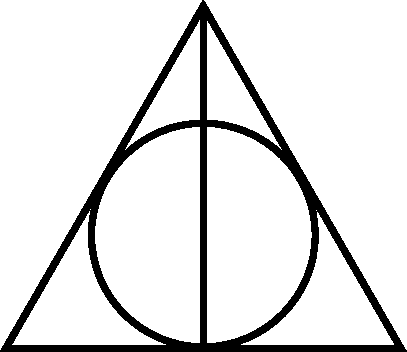
\includegraphics[scale=0.125]{images/Deathly_Hallows_Sign.pdf}
\end{center}
}
\vspace*{\fill}
\clearpage

%  LocalWords:  nd Kahneman eeeeviiil medi Hmmm stalkery
